\documentclass[class=article, crop=false, 12pt]{standalone}
\usepackage[subpreambles=true]{standalone}
\usepackage{../.common/common}


\author{Tony Shing}
%\pretitle{Supplementary}

\topic{Note 09 (Thermodynamics)}
\title{Thermodynamics Entropy}

\version{2025} % leave blank for omitting

\begin{document}

\maketitle


\begin{overview}
    \begin{itemize}
        \item Reversible Process v.s. Irreversible Process
        \item Related history of Thermodynamics entropy (anything before Boltzmann)
        \begin{itemize}
            \item Carnot's engine
            \item Kelvin's temperature
            \item Clausius' entropy function
        \end{itemize}
    \end{itemize}

\end{overview}




% content begins here
% Section %%%%%%%%%%%%%%%%%%%%%%%%%%%%%%%%%%%%%%%%%%%%%%%%%%%%
\section{Reversible v.s. Irreversible}

In thermodynamics, a system is undergoing a "reversible" process only if
\begin{itemize}
    \item No energy loss out of system (i.e. satisfy thermal \nth{1} law), and
    \item The process is quasi-static.
\end{itemize}

%%%%%%%%%%%%%%
\subsection{Quasi Static Process}

The term "\bf{quasi-static}" literally describes the system as looking like static,
but at the same time is also changing, 
like in a "half-equilibium-half-transititioning" state.
To understand why we need such definition,
we can look at the reality during the process of a gas compression.

\vskip 1em
\begin{minipage}{0.68\linewidth}
    \begin{enumerate}
        \item \ul{Before Compression}, 
        gas particles are evenly distributed.
        Particles' collisions are about the same everywhere in the container,
        so we can assign \cul[red]{a single well-defined value} as the pressure in the container.
    \end{enumerate}
\end{minipage}
\begin{minipage}{0.3\linewidth}
    \centering
    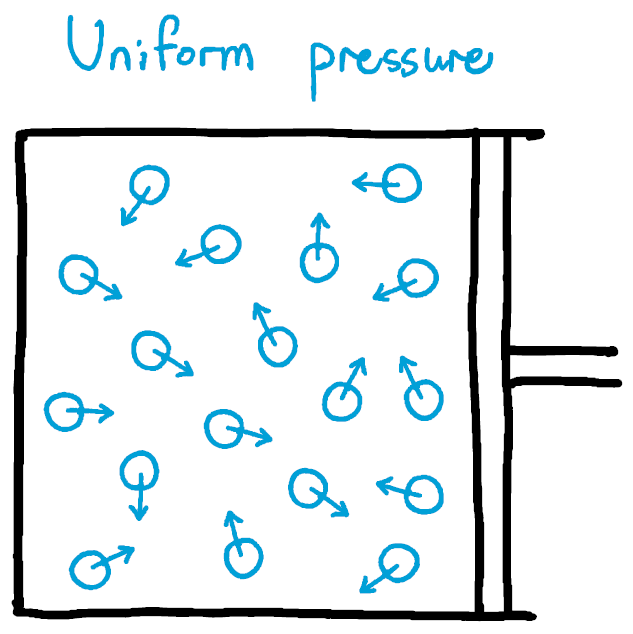
\includegraphics[height=9em]{compress1}
\end{minipage}

\vskip 1em
\begin{minipage}{0.68\linewidth}
    \begin{enumerate}
        \item[2.] \ul{Right at the beginning of the push}, 
        only particles near the piston can feel the piston pushing. 
        So region near the piston has a different pressure from region far away from the piston.
        The pressure in the container becomes ambiguous.
    \end{enumerate}
\end{minipage}
\hspace{0.01\textwidth}
\begin{minipage}{0.3\linewidth}
    \centering
    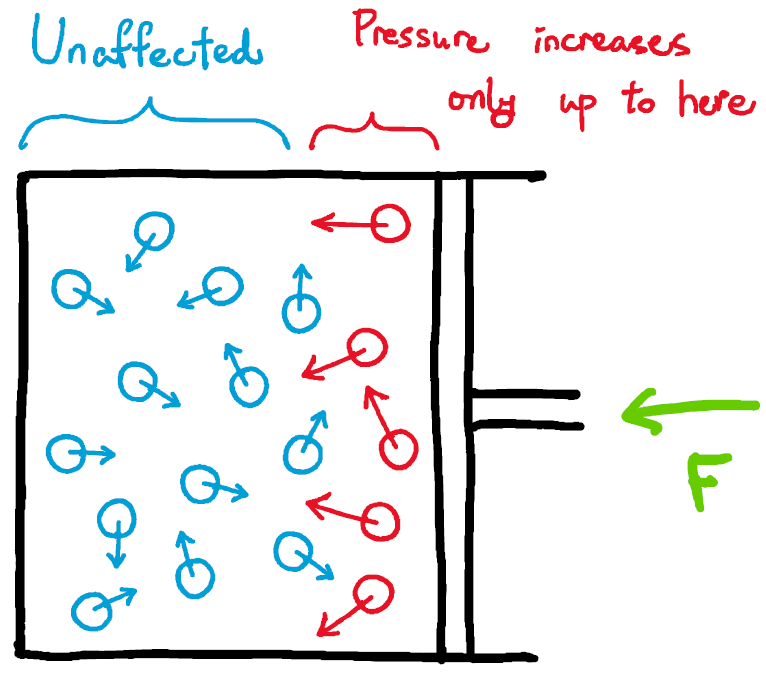
\includegraphics[height=9em]{compress2}
\end{minipage}

\begin{minipage}{0.68\linewidth}
    \begin{enumerate}
        \item[3.] \ul{When piston just comes to stop}, 
        particles pushed by piston start to mix with the rest of the gas particles.
        The pressure in the container is still ambiguous.
    \end{enumerate}
\end{minipage}
\hspace{0.01\textwidth}
\begin{minipage}{0.3\linewidth}
    \centering
    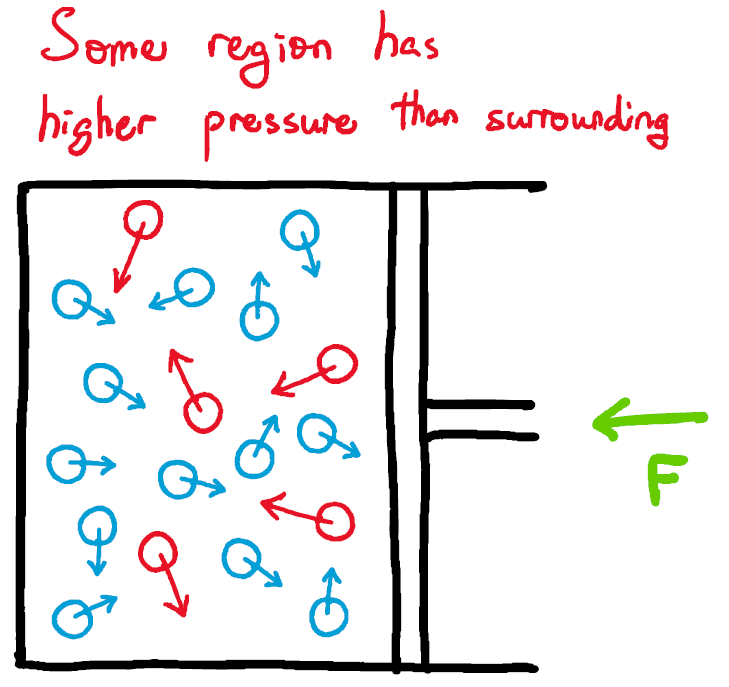
\includegraphics[height=9.5em]{compress3}
\end{minipage}

\vskip 1em
\begin{minipage}{0.67\linewidth}
    \begin{enumerate}
        \item[4.] \ul{After some time},
        particles become well-mixed and KE becomes evenly distributed.
        We can again assign a single well-defined value as the pressure in the container.
    \end{enumerate}
\end{minipage}
\begin{minipage}{0.3\linewidth}
    \centering
    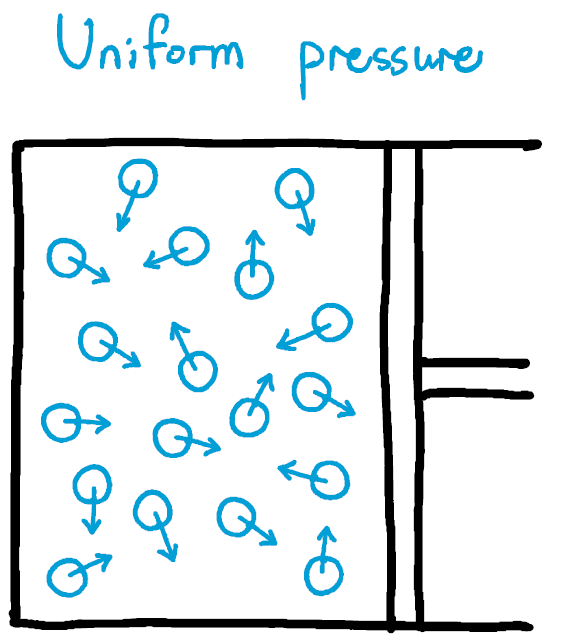
\includegraphics[height=9em]{compress4}
\end{minipage}

\vskip 2em
Now comes the problem: 
we cannot use a single value to represent the pressure during the compression. 
Is it really correct to represent a process with a single line in the PV diagram,
as we did in the last note?

\begin{center}
    \begin{minipage}{0.25\linewidth}
        \centering
        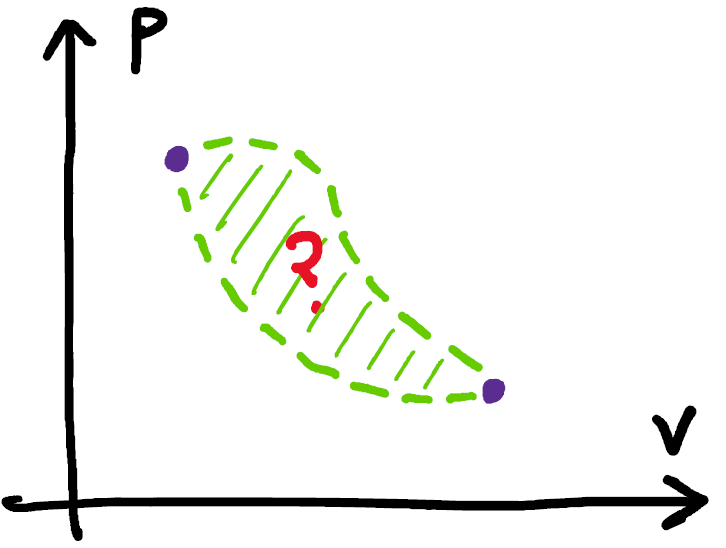
\includegraphics[width=\textwidth]{PV_inf4}
    \end{minipage}
    {\Large $\qquad=\qquad$}
    \begin{minipage}{0.25\linewidth}
        \centering
        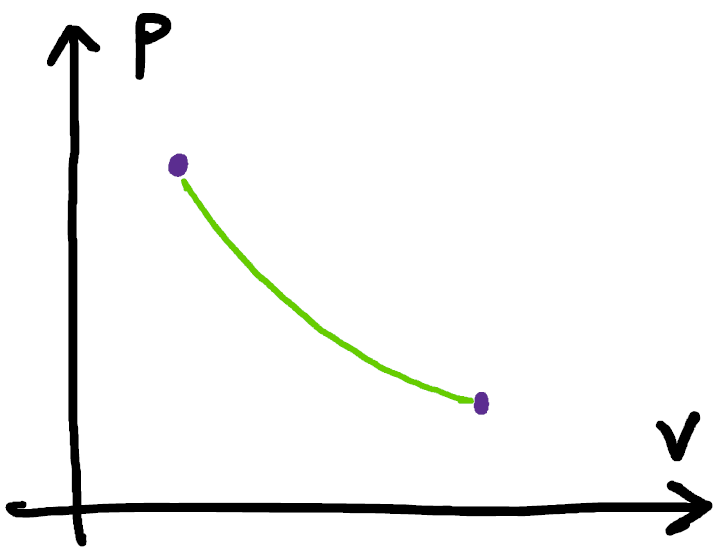
\includegraphics[width=\textwidth]{PV_inf3}
    \end{minipage}
    {\huge ?}
\end{center}

\vskip 1em
In reality, \red{this is indeed incorrect}.
But in order to use the derived results,
physicists theorize the process to be "infinitestimal":
\begin{itemize}
    \item The piston is moving extremely slow,
    only compress a very tiny volume at each step.
    
    \item Time allowed for the gas to fully mix is extremely long. 
    So we can assure the pressure have enough time to distribute evenly. 
\end{itemize}

When such step is repeated for many many times, 
we can "approximate" the state parameters to be well-defined and changing continuously along the process,
by having many intermediate states in between.

\begin{center}
    \begin{minipage}{0.25\linewidth}
        \centering
        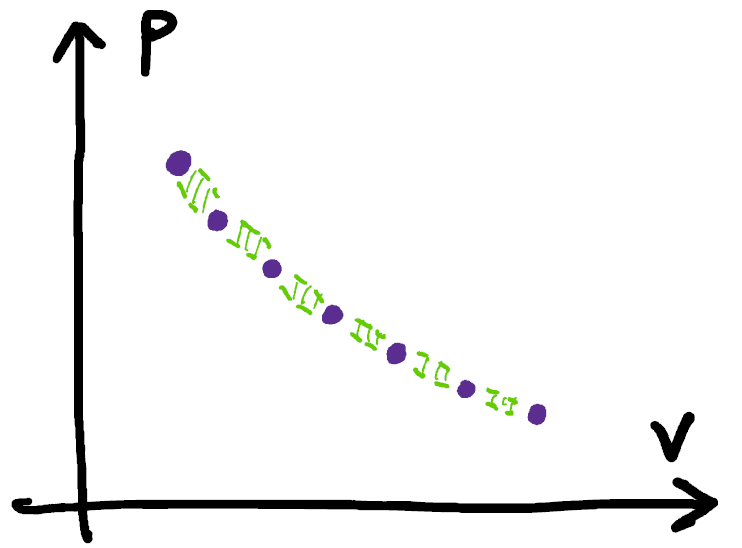
\includegraphics[width=\textwidth]{PV_inf1}
    \end{minipage}
    {\Large $\qquad \approx \qquad$}
    \begin{minipage}{0.25\linewidth}
        \centering
        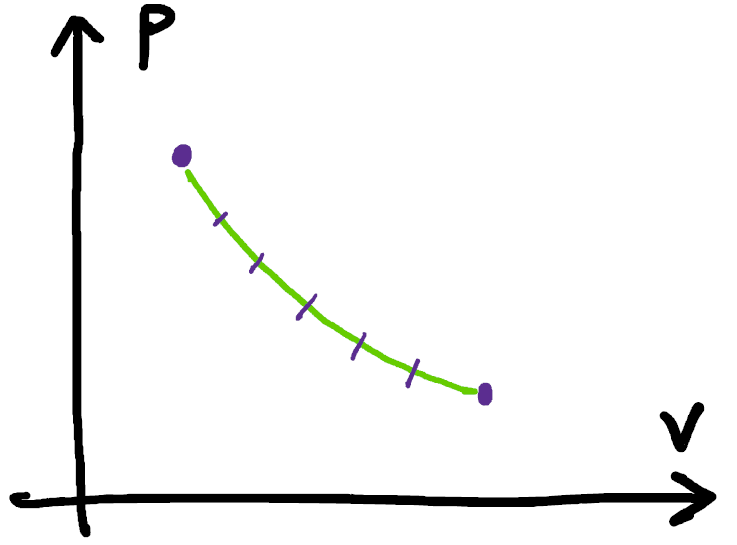
\includegraphics[width=\textwidth]{PV_inf2}
    \end{minipage}
\end{center}


Such process is called "Quasi-Static" process:
\aleq{
    \text{Quasi-static } = 
    \tkn{half_eqm}{\cul[red]{\text{Half Equilibrium }}}
    + \tkn{half_tran}{\cul[blue]{\text{ Half transitioning}}}
}
\addArrow[red]{half_eqm}{(-10ex,-3ex)}
{Made of infinitely many intermediate states\\so its state parameters are\\always well-defined}
{(0,-2ex)}{(0,-3.5ex)}
\addArrow[blue]{half_tran}{(10ex,-3ex)}
{Made of infinitely many processes\\so state parameters are\\always smoothly changing}
{(0,-2ex)}{(0,-3.5ex)}

\vskip 4em

Quasi-static processes are the ideal processes in thermodynamics because they are \cul[red]{reversible}.

\begin{center}
    \begin{minipage}{0.15\linewidth}
        \centering
        \hspace{2em}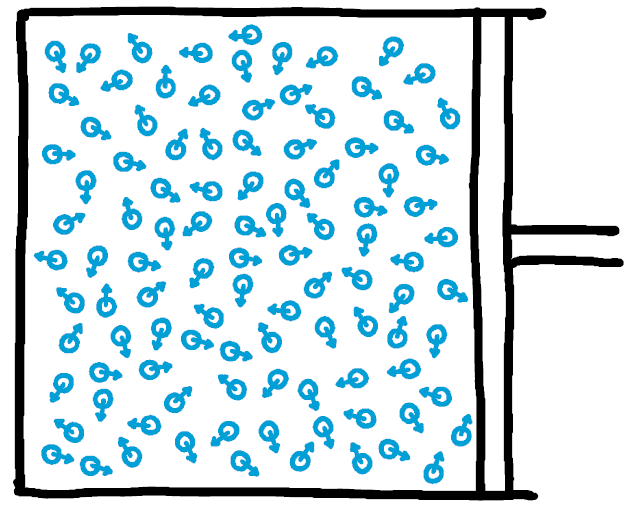
\includegraphics[height=5.5em]{quasi1}
        {\scriptsize \phantom{abc}\\[-1ex]\phantom{abc}}
    \end{minipage}
    \quad\  $\mstack{\Rightarrow\\\phantom{a}}$\quad 
    \begin{minipage}{0.23\linewidth}
        \centering
        \hspace{3em}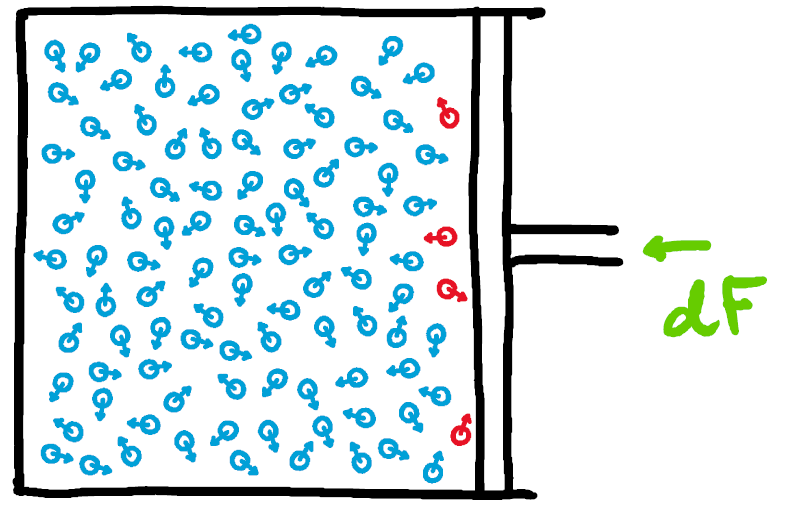
\includegraphics[height=5.5em]{quasi2}\\
        {\scriptsize A small push only affects\\[-1ex]very few particles}
    \end{minipage}
    $\mstack{\Rightarrow\\\phantom{a}}$
    \begin{minipage}{0.23\linewidth}
        \centering
        \hspace{2em}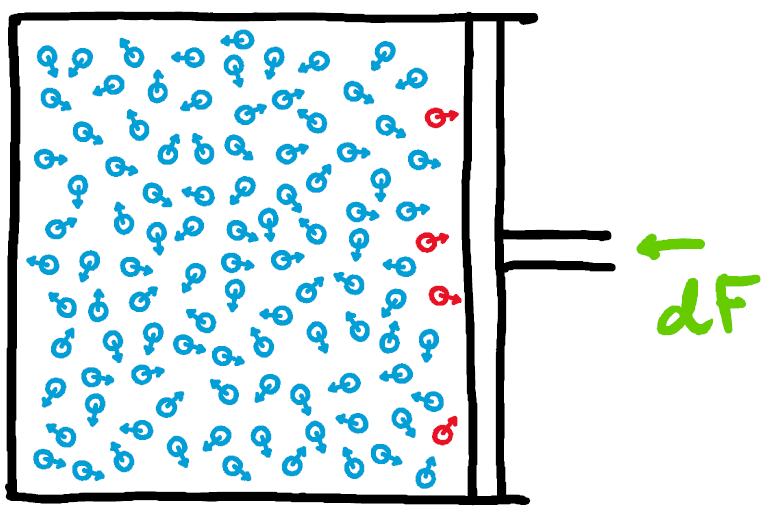
\includegraphics[height=5.5em]{quasi3}\\
        {\scriptsize The particles counter\\[-1ex]strike the piston}
    \end{minipage}
    $\mstack{\Rightarrow\\\phantom{a}}$\quad\quad
    \begin{minipage}{0.15\linewidth}
        \centering
        \hspace{2em}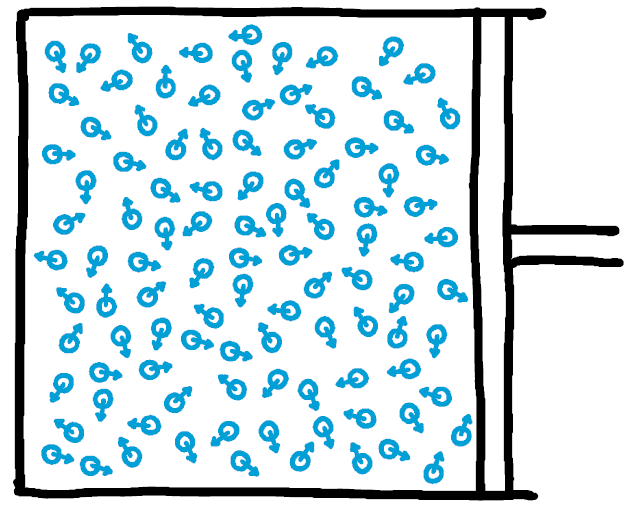
\includegraphics[height=5.5em]{quasi1}\\
        {\scriptsize Restore\\[-1ex]\phantom{abc}}
    \end{minipage}
\end{center}


%%%%%%%%%%%%%%
\subsection{Irreversible Process}

However, quasi-static process is impractical because
\begin{itemize}
    \item it takes an extremely long waiting time (ideally, infinite long).
    \item only very small change at each step (ideally, infinitestimally small).
\end{itemize}

\red{All thermodynamics processes, when carried out in reality, are irreversible.}
The lines in the P-V diagram shall not be as well-defined as we have seen.
Adapting this reality to what we have learnt in the last note,
\begin{enumerate}
    \item Formula to $\var{W}$ and $\var{Q}$ are only for the ideal reversible case. 
    An irreversible process does not have a not well-defined path, so integration is not analytically comput-able.
    \aleq{
        \int_{\substack{\text{Irreversible}\\\text{process}}} \var{W} 
        = \int_\red{\substack{\text{No exact}\\\text{path}}} \dd{W} 
        = \qty(\text{Uh oh...})
    }

    \item A real engine cannot be run as a refridgerator by inverting its cycle, 
    because its processes are no longer reversible.

    \item Efficiency of real engines must be less than the theoretical limit (Carnot's theorem).
    
    
    
\end{enumerate}

\begin{notation}[Side Note:]
    Irreversibility only happens in the thermodynamics pespective.\\

    In mechanical perspective, 
    state parameters are positions and velocities of the particles $(x_i, v_i)$
    which are continuous and well-defined all the time
    because they can be predicted by Newton's \nth{2} law.
    We can tell when the system will return to its original state.\\

    In the next note, we shall discuss the differences between mechanical and thermodynamics perspectives,
    and how do these lead to irreversibility of a system.
\end{notation}



\linesep
% Section %%%%%%%%%%%%%%%%%%%%%%%%%%%%%%%%%%%%%%%%%%%%%%%%%%%%
\section{Historical Development of Thermodynamics \nth{2} Law}

The following sections present several important discoveries within the early period of thermodynamics researches.
\begin{itemize}
    \item (1824) Carnot's theorem and Carnot's engine.
    \item (1848) Kelvin temperature scale.
    \item (1850-1851) First two statements of thermodynamics \nth{2} law by Kelvin and Clausius.
    \item (1854) First mathematical formulation of entropy by Clausius.
\end{itemize}

The era of classical thermodynamics ended around 1860s, 
when \it{statistical mechanics} started taking place. 

%%%%%%%%%%%%%%
\subsection{Carnot's Engine \& Carnot's Theorem}

\href{https://en.wikipedia.org/wiki/Nicolas_L\%C3\%A9onard_Sadi_Carnot}{Nicolas Léonard Sadi Carnot}
was the first person who suggested the concepts of \bf{heat engine}:
\begin{itemize}
    \item One can extract energy for our use, via the process when heat flow from hot object to cold object.
    It is just like we can extract KE from objects that fall from a high place to low place.

    \item A heat engine is a operator that runs \cul[red]{cyclic} processes which can extract energy to do work, 
    from the natural heat flow between hot and cold objects.

    \item As long as the temperature difference between hot/cold objects is maintained,
    a heat engine can run a cycle of processes indefinitely. 
\end{itemize}



He also proposed one of the foundation in thermodynamics: \bf{Carnot's theorem}.
\quoting{
    Among any heat engines that operate between 2 heat reservoirs of fixed temperature, 
    the engine that runs reversible processes is the most efficient in converting heat to work done.
}

The reversible engine that he proposed was the Carnot engine, 
which \bf{limits the theoretical maximum of engine efficiency for any engines that operate between two fixed temperatures}.
Any other engines that run reversible cycles would also have the same efficiency.

\begin{center}
    \begin{minipage}{0.5\linewidth}
        \centering
        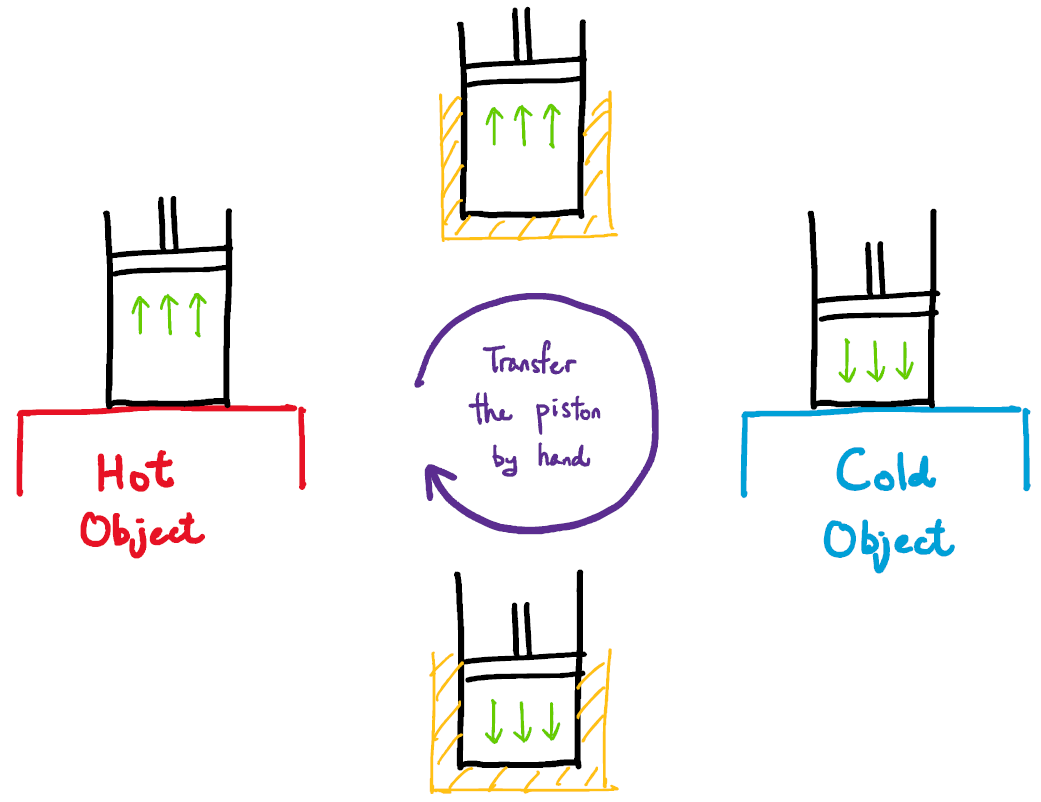
\includegraphics[width=\textwidth]{carnot_piston}
    \end{minipage}
    \hspace{0.05\textwidth}
    \begin{minipage}{0.3\linewidth}
        \centering
        This is the original proposal of Carnot engine.
    \end{minipage}
\end{center}

\begin{center}
    \begin{minipage}{0.4\linewidth}
        \begin{tabular}{>{\centering\arraybackslash}m{3cm} >{\centering\arraybackslash}m{3cm}}
            & Process
            \\
            \hline
            \cbox[blue]{1} $\rightarrow$ \cbox[blue]{2}
            & Iso. T
            \\
            \hline
            \cbox[blue]{2} $\rightarrow$ \cbox[blue]{3}
            & Adiabetic
            \\
            \hline
            \cbox[blue]{3} $\rightarrow$ \cbox[blue]{4}
            & Iso. T
            \\
            \hline
            \cbox[blue]{4} $\rightarrow$ \cbox[blue]{1}
            & Adiabetic
        \end{tabular}
    \end{minipage}
    \hspace{0.05\textwidth}
    \begin{minipage}{0.3\linewidth}
        \centering
        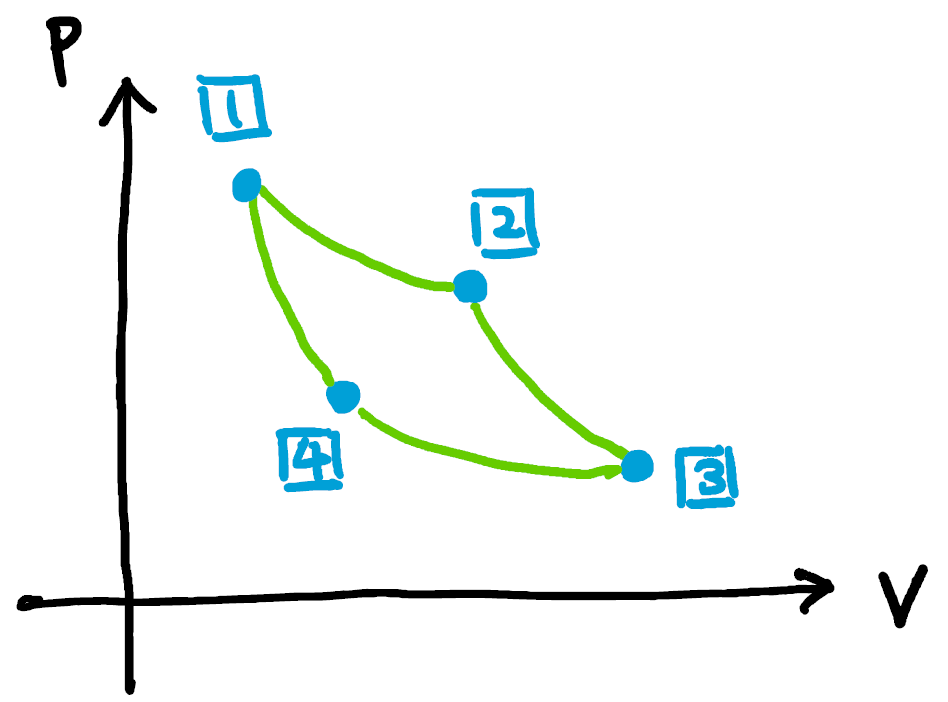
\includegraphics[width=\textwidth]{carnot_cycle}
    \end{minipage}
\end{center}

Unfortunately, Carnot did not prove his theorem correctly - 
his arguments were based on thermal \nth{1} law and involved circular reasoning. 
He passed away in 1832 and did not live long enough to see his work being recognized.\\

It was until around 1850s, 
scientists realized that Carnot's theorem shall not be proven by \nth{1} law.
It must be described as an independent law - the thermodynamics \nth{2} law.

\vskip 1em
\begin{notation}[Side note:]
    \begin{itemize}
        \item Theorem = Consequences that can be logically derived from known facts.
        \item Law = Rules that are concluded based on observations (like common sense).\\ 
        \phantom{Law =} Such observations may be explanable with deeper theories,\\
        \phantom{Law =} but we do not know yet.
    \end{itemize}
\end{notation}



%%%%%%%%%%%%%%
\subsection{The First 2 statements of Thermodynamics \nth{2} Law}

\href{https://en.wikipedia.org/wiki/Lord_Kelvin}{Lord Kelvin} 
and 
\href{https://en.wikipedia.org/wiki/Rudolf_Clausius}{Rudolf Clausius} 
independently formulated their own statement
about the law of irreversibility:
\begin{itemize}
    \item \ul{Kelvin}: No W.D. $\Rightarrow$ No reverse heat flow
    \item \ul{Clausius}: Cannot convert 100\% Heat flow to W.D.
\end{itemize}

Note that their statements are still "laws" - 
they were written down based on common sense, without explanation.\\

We can prove that they are logically equivalent to Carnot's theorem by contradiction 
(If one fails, the other must also fail.)

\begin{enumerate}
    \item \ul{Clausius fails $\Rightarrow$ Kelvin fails}\\
    Suppose Clausius' statement is wrong - 
    \it{there exists an engine that can convert 100\% of a heat flow to W.D.}

    \begin{center}
        \begin{minipage}{0.25\linewidth}
            \centering
            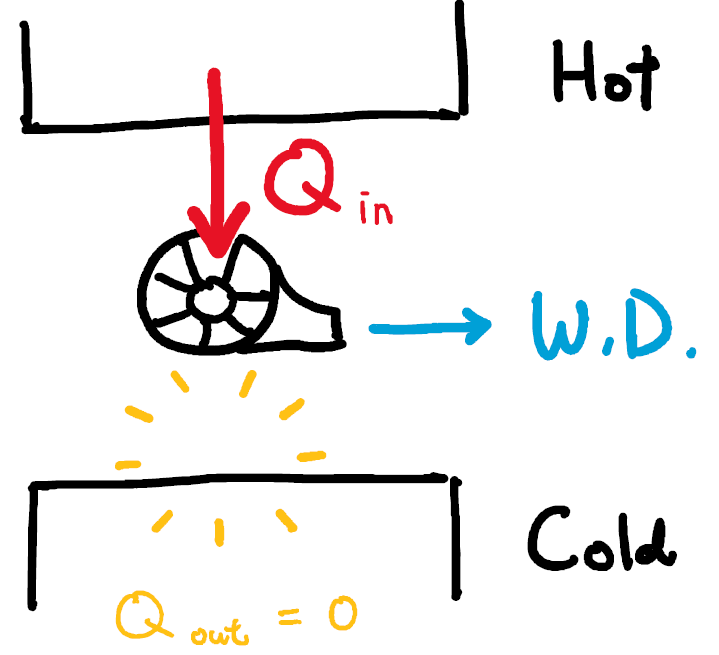
\includegraphics[width=\textwidth]{clausius1}
        \end{minipage}
    \end{center}

    Then we can operate it together with a refridgerator that runs Carnot cycle:

    \begin{center}
        \begin{minipage}{0.45\linewidth}
            \centering
            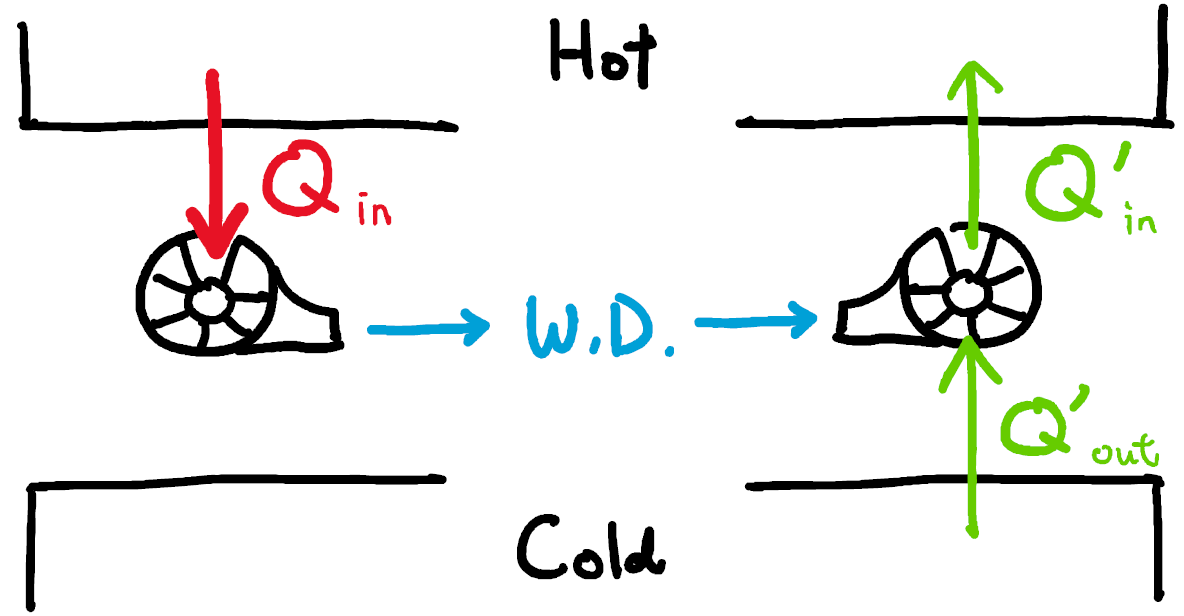
\includegraphics[width=\textwidth]{clausius2}
        \end{minipage}
    \end{center}

    By energy conservation, we have
    \aleq{
        Q'_\text{in} = Q'_\text{out} + \text{W.D.} = Q'_\text{out} + Q_\text{in} > Q_\text{in}
    }

    which is equivalent to a cycle with net heat flow of $Q'_\text{out}$ from colder reservoir to hotter reservoir,
    without any external W.D. supply. 
    \it{This is a contradiction to Kelvin's statement}.

    \begin{center}
        \begin{minipage}{0.4\linewidth}
            \centering
            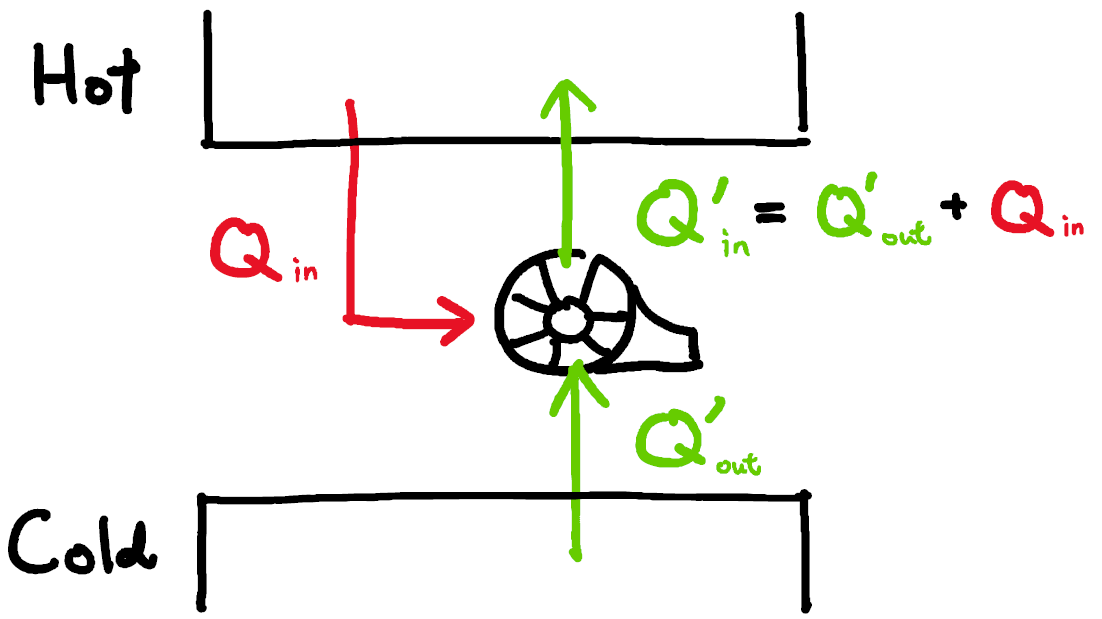
\includegraphics[height=9em]{clausius3}
        \end{minipage}
        \qquad{\huge$\equiv$}\qquad
        \begin{minipage}{0.3\linewidth}
            \centering
            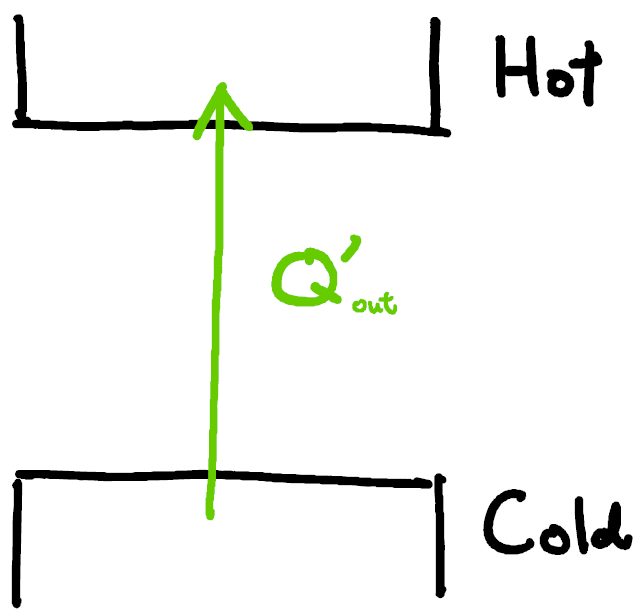
\includegraphics[height=9em]{clausius4}
        \end{minipage}
    \end{center}


    \vskip 1em
    \item \ul{Kelvin fails $\Rightarrow$ Clausius fails}\\
    Suppose Kelvin's statement is wrong -
    \it{heat can flow from a colder reservoir to a hotter reservoir without needing any external W.D.}

    \begin{center}
        \begin{minipage}{0.25\linewidth}
            \centering
            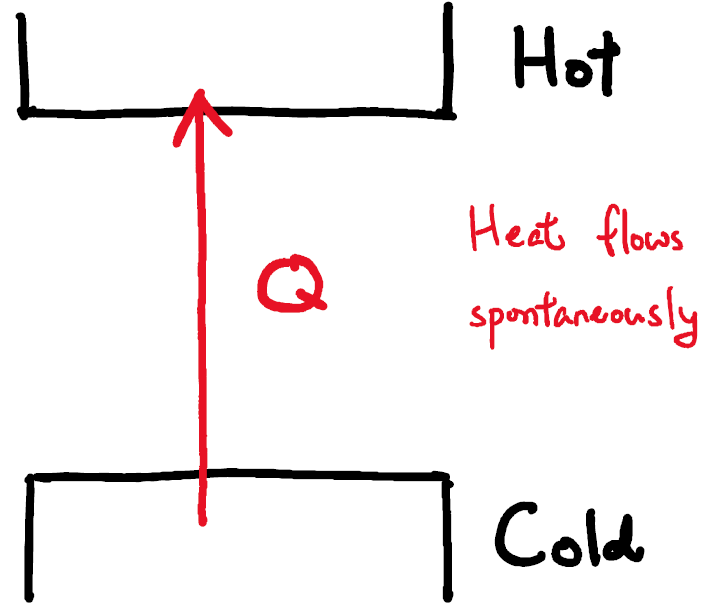
\includegraphics[width=\textwidth]{kelvin1}
        \end{minipage}
    \end{center}

    Then we can operate it together with an engine that runs Carnot cycle:

    \begin{center}
        \begin{minipage}{0.5\linewidth}
            \centering
            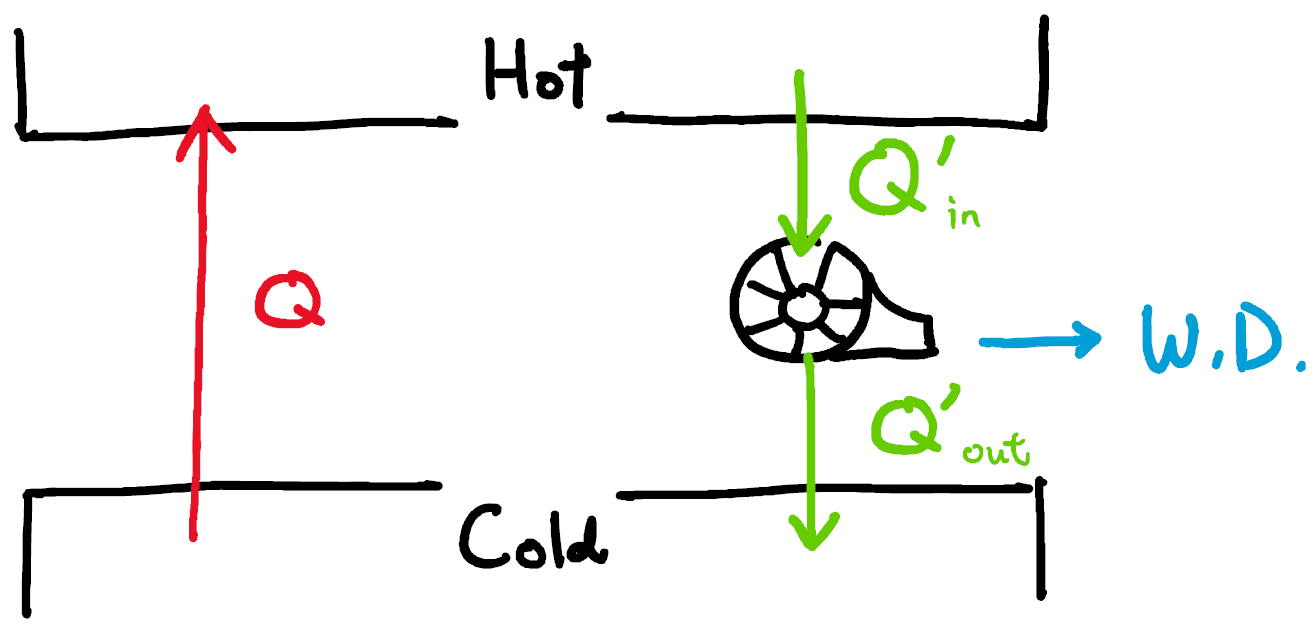
\includegraphics[width=\textwidth]{kelvin2}
        \end{minipage}
    \end{center}

    We can maintain the heat flow out of colder reservoir ($Q$) to equal to the heat flow into the colder reservoir ($Q'_\text{out}$),
    such that temperature of cold reservoir is kept constant. 
    By energy conservation we writes
    \aleq{
        Q = Q'_\text{out} = Q'_\text{in} - \text{W.D.}
    }

    which is equivalent to having 100\% of the heat extracted from hot reservoir to be converted into W.D..
    \it{This is a contradiction to Clausius' statement}.

    \begin{center}
        \begin{minipage}{0.4\linewidth}
            \centering
            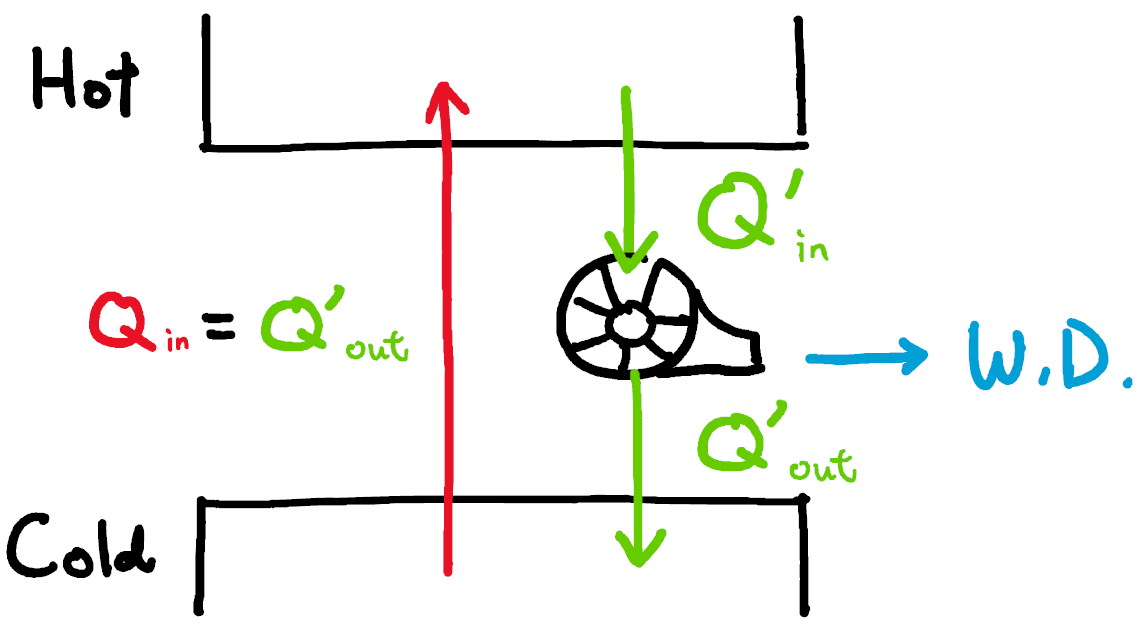
\includegraphics[height=9em]{kelvin3}
        \end{minipage}
        \qquad{\huge$\equiv$}\qquad
        \begin{minipage}{0.3\linewidth}
            \centering
            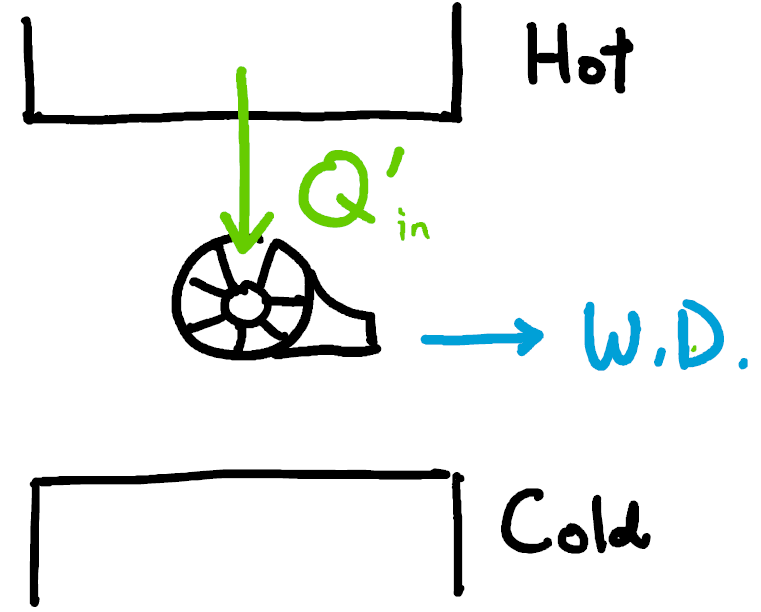
\includegraphics[height=9em]{kelvin4}
        \end{minipage}
    \end{center}


    \vskip 1em
    \item \ul{Clausius fails $\Rightarrow$ Carnot fails}\\
    This is automatically proven, since Clausius's statement failing means that 
    there exists an engine of 100\% efficiency,
    contradicted to the maximum limit of Carnot engine.

    \begin{center}
        \begin{minipage}{0.25\linewidth}
            \centering
            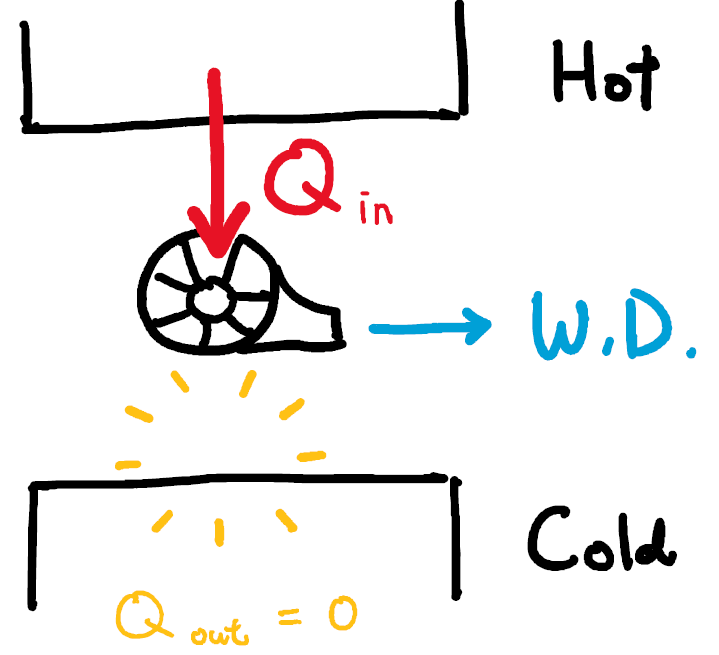
\includegraphics[width=\textwidth]{clausius1}
        \end{minipage}
        \qquad$\Rightarrow$\qquad
        Efficiency $= \dfrac{\text{W.D.}}{Q_\text{in}} = 100\%$ 
    \end{center}


    \vskip 1em
    \item \ul{Carnot fails $\Rightarrow$ Kelvin fails}\\
    Suppose Carnot's theorem is wrong - 
    \it{there is a hypothetical engine that runs irreversible process but has a higher efficiency than a Carnot engine}.
    \aleq{
        \qty(\mstack{\text{Efficiency of}\\\text{Hypothetical engine}})\ =\ \eta_1
        > \eta_2
        \ =\ \qty(\mstack{\text{Efficiency of}\\\text{Carnot engine}})
    }

    Then we can operate it together with a Carnot refridgerator.

    \begin{center}
        \begin{minipage}{0.8\linewidth}
            \centering
            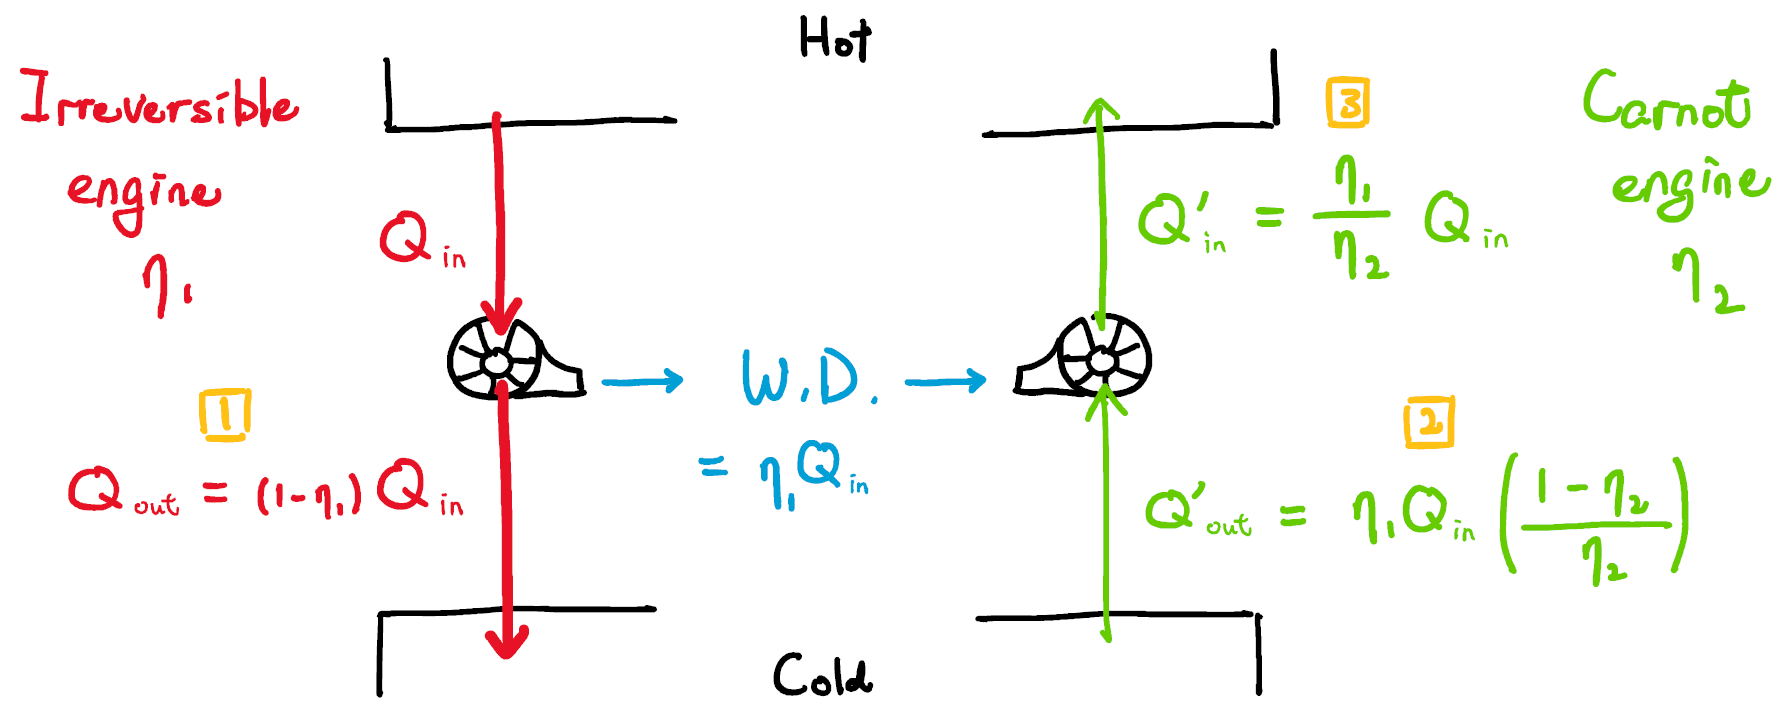
\includegraphics[width=\textwidth]{carnot_clausius}
        \end{minipage}
    \end{center}

    If we look at the net heat flow into the hot reservoir,
    \begin{enumerate}
        \item[1.] Heat $Q_\text{in}$ is input into the irreversible engine of efficiency $\eta_1$.
        So amount of heat converted to W.D. $=\eta_1Q_\text{in}$.

        \item[2.] Reversible engine of efficinency $\eta_2$ can be reverted into a refridgerator of COP $=\qty(\frac{1-\eta_2}{\eta_2})$.
        Amount of heat removed from cold reservoir $=\text{W.D.}\times \text{COP} = \eta_1Q_\text{in}\qty(\frac{1-\eta_2}{\eta_2})$.

        \item[3.] Total heat returning to hot reservoir $= \eta_1Q_\text{in} + \eta_1Q_\text{in}\qty(\frac{1-\eta_2}{\eta_2}) = \frac{\eta_1}{\eta_2} Q_\text{in}$.
        
    \end{enumerate}
    Observing that 
    \aleq{
        \qty(\mstack{\text{Heat flow into}\\\text{hot reservoir}}) - \qty(\mstack{\text{Heat flow out of}\\\text{hot reservoir}})
        \ =\ \frac{\eta_1}{\eta_2}Q_\text{in} - Q_\text{in} >0  \quad\text{ if }\quad{\eta_1>\eta_2}
    }

    which is equivalent to having heat flowing from cold reservoir to hot reservoir spontaneously.
    \it{This is a contradiction to Kelvin's statement}.\\

    \bf{\ul{Note}}: Because an irreversible engine cannot be reverted to become an irreversible refridgerator,
    It is not logical to operate an irreversible engine side by side with an irreversible refridgerator to keep the heat balance.

   

\end{enumerate}



\linesep
%%%%%%%%%%%%%%
\section{Kelvin's Temperature Scale}

\subsection{Temperature Measurement Before \nth{19} Century}

The oldest temperature scales were defined using interpolation between two reference points.
For example, the Celsius scale was defined by the expansion in length of mercury/alcohol in a thin glass tube,
using water's freezing and boiling as reference points and divide into 100 grids.\\

Meanwhile, thermodynamics properties of ideal gas were already well-investigated through experiments.
For example, scientists already knew that the P-T relation is linear,
i.e. it can be plotted as a straight line.

\begin{center}
    \begin{minipage}{0.8\linewidth}
        \centering
        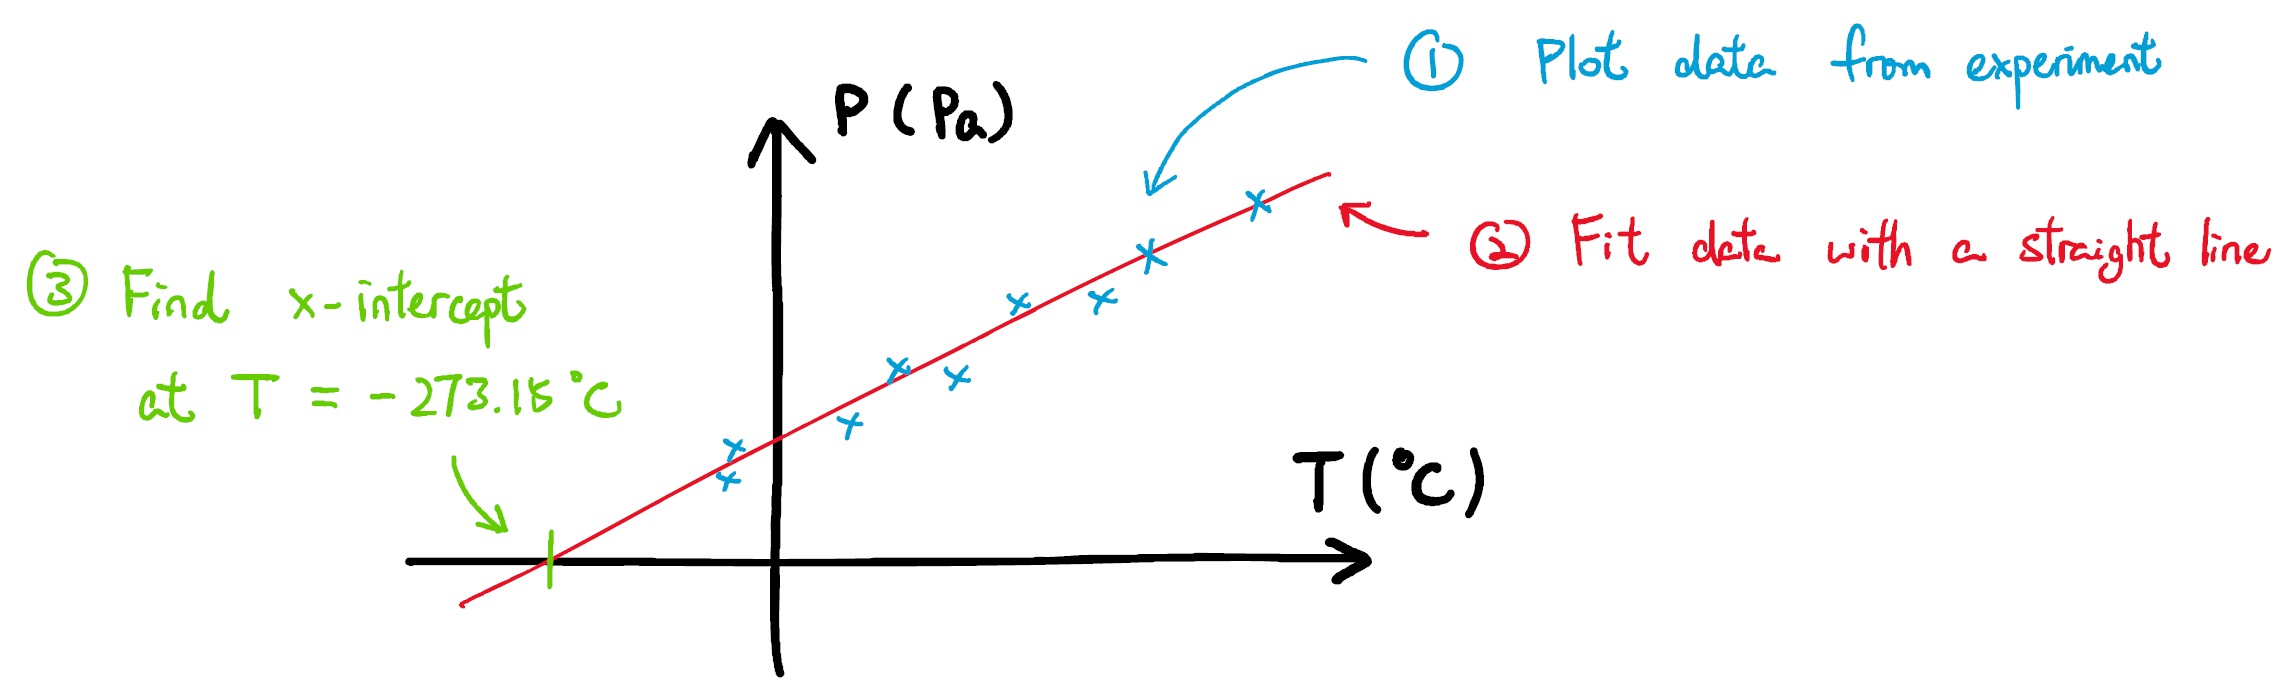
\includegraphics[width=\textwidth]{temp_inter}
    \end{minipage}
\end{center}

However, data were limited by the freezing point of material in the thermometer.
Without experimental support, it was impossible to tell if there were new physics beyond $-273.15^\circ$C.


%%%%%%%%%%%%%%
\subsection{Thermodynamics Temperature Scale}

The Kelvin temperature scale is not just naively shifting the $0$ point from $0^\circ$C to $-273.15^\circ$C,
but is a theoretical scale based on the efficiency of Carnot engine.
\aleq{
    \eta &= 1 - \frac{Q_C}{Q_H}
    = 1 - \frac{\text{Heat input to colder reservoir}}{\text{Heat output from hotter reservoir}}\\[1em]
    &\sim 1- \frac{T_C}{T_H}
    = 1 - \frac{\text{How cold is the colder reservoir}}{\text{How hot is the hotter reservoir}}\\[1em]
    &=\qty(\mstack{\text{Some function of "\bf{\red{Relative hottness}}"}\\[0.5ex]\text{between hotter and colder reservoir}})
    %&= f\qty(\mstack{\text{Some function of}\\\text{how hot the hotter reservoir}\\\text{is relative to}\\\text{the colder reservoir}})
}

The idea is that in a reversible engine, 
the engine efficiency is purely determined by how hot the hotter reservoir relative to the colder reservoir.
If we can measure the engine efficiency, 
we can create a scale of hottness between reservoirs.

\begin{center}
    \begin{minipage}{0.7\linewidth}
        \centering
        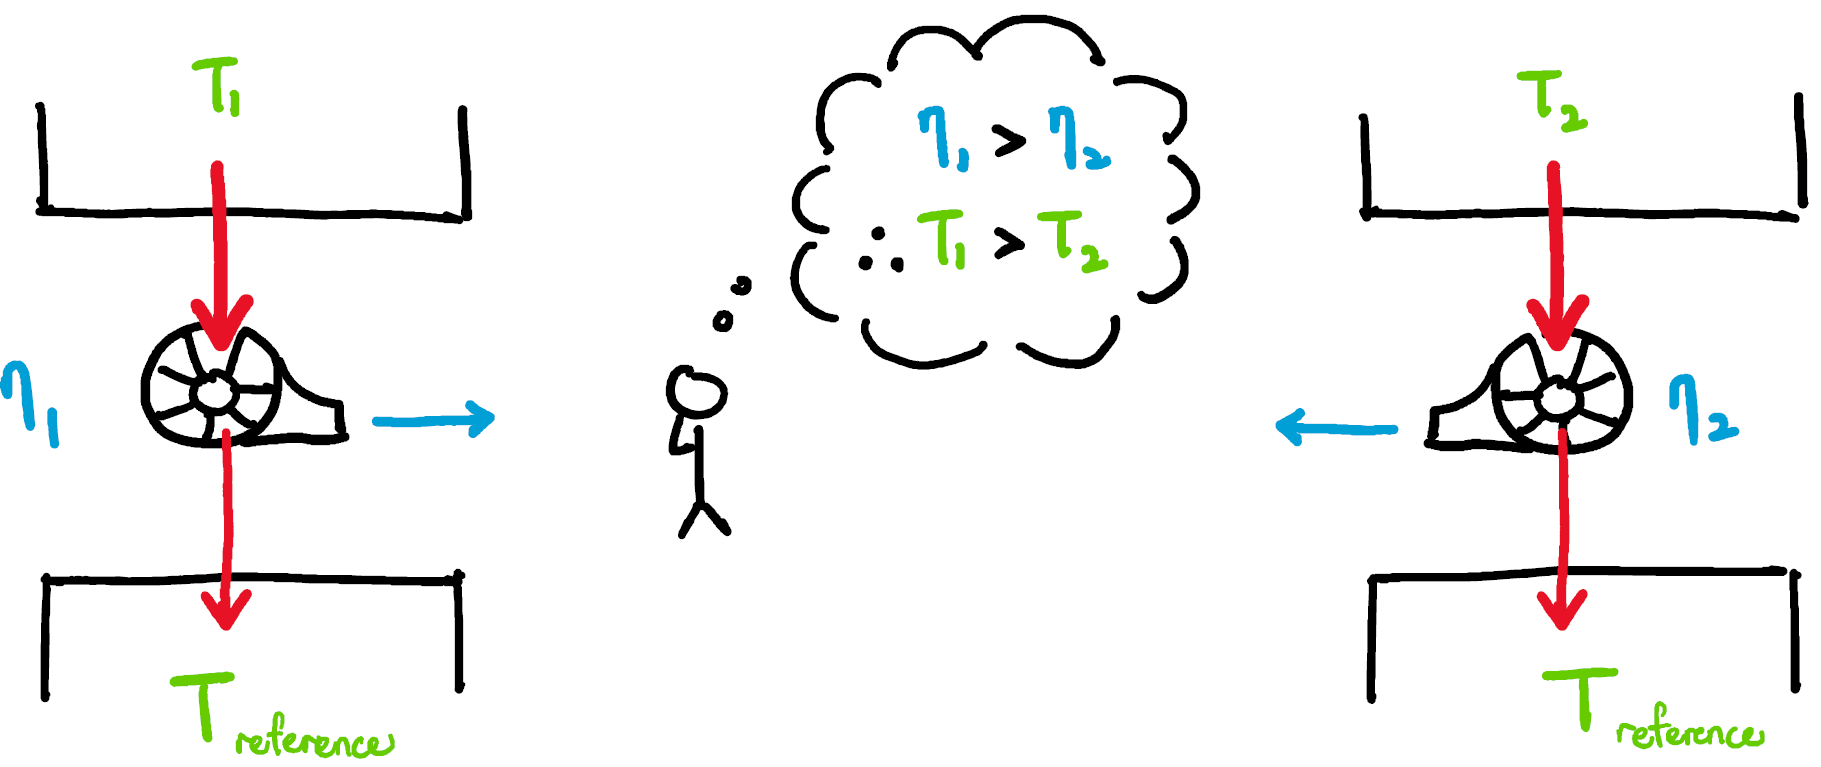
\includegraphics[width=\textwidth]{temp_eff}
    \end{minipage}
\end{center}


Suppose we measure the "hottness" of 2 heat reservoirs $H$ and $C$ \cul[red]{using a new scale $\theta$}.
Quantify their "hottness" to be some numbers $\theta_H$ and $\theta_C$ respectively.

\vskip 1em
\begin{minipage}{0.6\linewidth}
    \begin{enumerate}
        \item Operate a Carnot engine between the two reservoirs.
        Let the efficiency to be some function of $\theta_H$ and $\theta_C$.
        \aleq{
            \eta = 1-\frac{Q_C}{Q_H} = 1- f(\theta_C, \theta_H)
        }
    \end{enumerate}
\end{minipage}
\hspace{0.05\textwidth}
\begin{minipage}{0.3\linewidth}
    \centering
    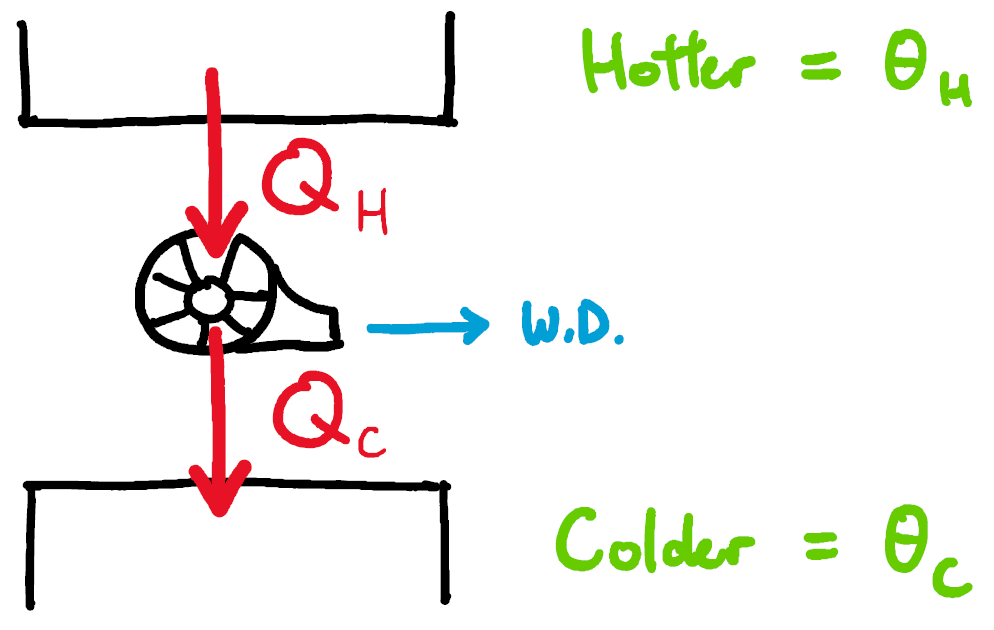
\includegraphics[width=\textwidth]{temp_engine1}
\end{minipage}

\vskip 1.5em
\begin{enumerate}
    \item[2.] Observe that $f$ needs to satisfy these mathematical relations:
    \begin{itemize}
        \item $\dfrac{Q_C}{Q_H} = \dfrac{Q_C}{Q_W}\cdot \dfrac{Q_W}{Q_H} 
            \quad\Rightarrow\quad f(\theta_C,\theta_H) = f(\theta_C, \theta_W)\cdot f(\theta_W, \theta_H)$

        \vskip 1em
        \item $\dfrac{Q_C}{Q_H} = \dfrac{1}{\frac{Q_H}{Q_C}}
            \quad\Rightarrow\quad f(\theta_C, \theta_H) = \dinv{f(\theta_H, \theta_C)}$
    \end{itemize}

    \newpage
    \item[3.] What kinds of function $f(\cdot,\cdot)$ satisfy these relations?
    Although we may naively take $f(\theta_C,\theta_H) = \frac{\theta_C}{\theta_H}$,
    there are in fact infinitely many choices. For example,

    \begin{itemize}
        \item Taking $f(\theta_C,\theta_H) = \dfrac{\theta_C}{\theta_H}$, then
        \aleq{
            f(1,10) = \frac{1}{10} = \frac{10}{100} = f(10,100)
        }
        An engine working between reservoirs with "hottness" 1 and 10 yield the same efficiency
        as working between reservoirs with "hottness" 10 and 100.

        \begin{center}
            \begin{minipage}{0.5\linewidth}
                \centering
                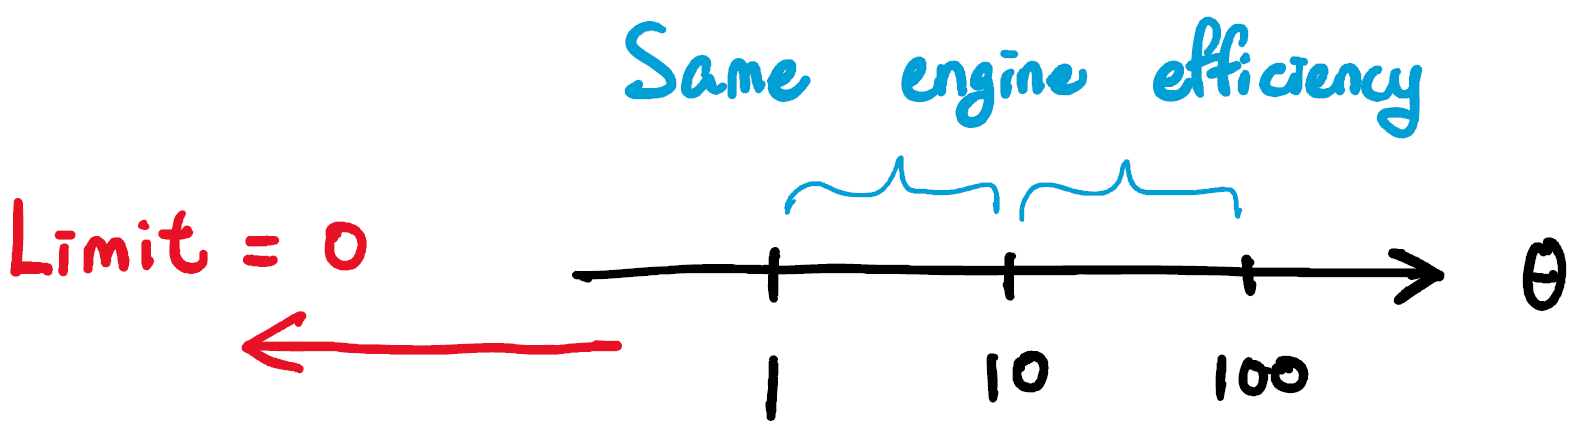
\includegraphics[width=\textwidth]{temp_scale_log}
            \end{minipage}
        \end{center}

        \ul{This scale of hottness is a logarithmic scale relative to efficiency}.

        \vskip 2em
        \item Taking $f(\theta_C,\theta_H) = e^{\theta_C - \theta_H}$, then
        \aleq{
            f(0,10) = e^{10-0} = e^{20-10} = f(10,20)
        }
        An engine working between reservoirs with "hottness" 0 and 10 yield the same efficiency
        as working between reservoirs with "hottness" 10 and 20.

        \begin{center}
            \begin{minipage}{0.5\linewidth}
                \centering
                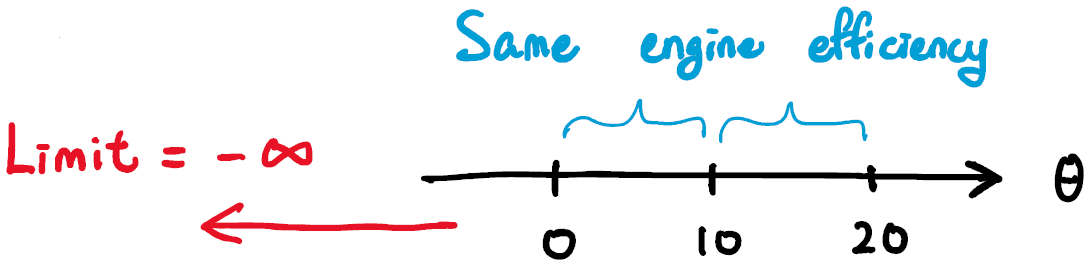
\includegraphics[width=\textwidth]{temp_scale_lin}
            \end{minipage}
        \end{center}

        \ul{This scale of hottness is a linear scale relative to efficiency}.

    \end{itemize}

    \vskip 1em
    \item[4.] Because the Celcius scale already existed at that time
    and was widely used in thermodynamics experiment and theories, 
    such as deriving the efficiency of Carnot engine,
    \aleq{
        \mstack{\text{Carnot engine's}\\\text{efficiency}} = 1-\frac{T_L+273.15}{T_H+273.15}
    }

    where $T_H, T_L$ are values of temperature measured under the Celcius scale.
    It is just convenient to choose $f(\theta_1,\theta_2) = \dfrac{\theta_1}{\theta_2}$ so that our new scale of hottness is
    \aleq{
        \Aboxed{
            \theta = \qty(\text{Celsius temperature}) + 273.15
        }
    }
    which is now known as the \bf{Kelvin temperature scale}.


\end{enumerate}

%%%%%%%%%%%%%%
\subsection{The Consequence: Absolute Zero}

Through the Kelvin scale,
we can relate temperature with engine efficiency to explain why the \red{absolute zero temperature cannot be reached}. 
Consider a Carnot engine working between two reservoirs,
with the colder side at absolute zero ($\theta=0$).
Then the efficiency of this engine is

\begin{center}
    \begin{minipage}{0.3\linewidth}
        \aleq{
            \eta = 1 - \frac{0}{\theta_H} = 1
        }
    \end{minipage}
    \hspace{0.05\textwidth}
    \begin{minipage}{0.3\linewidth}
        \centering
        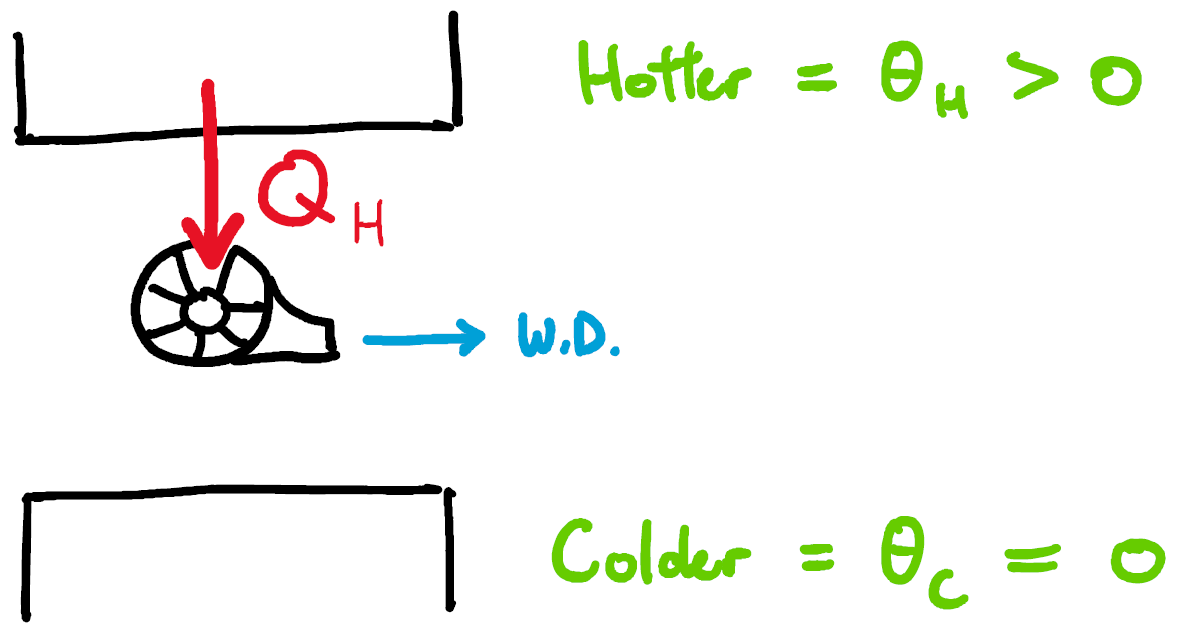
\includegraphics[width=\textwidth]{temp_0K}
    \end{minipage}
\end{center}

100\% of the heat is converted into work done,
which is a violation to the Clausius statement.\\

In addition, if we choose a different temperature scale 
\begin{itemize}
    \item Choose $f(\theta_C,\theta_H) = \dfrac{\theta_C}{\theta_H}$ \quad$\Rightarrow$\quad 
    The point of $100\%$ efficiency corresponds to $\theta_C=0$.

    \item Choose $f(\theta_C,\theta_H) = e^{\theta_C - \theta_H}$ \quad$\Rightarrow$\quad 
    The point of $100\%$ efficiency corresponds to $\theta_C=-\infty$.
\end{itemize}

\vskip 1ex
So you may also claim that negative temperature is not physical because of our choice of scale. 



\linesep
%%%%%%%%%%%%%%
\section{Clausius's Entropy Function}

The term "\bf{entropy}" was named by Rudolf Clausius to a special state function $S$
\aleq{
    \dd{S} \ \defeq\ \frac{\var{Q}_\green{\text{in}}}{T} 
}

Here the $Q$ are labeled $Q_\green{\text{in}}$ only to emphasize that 
$Q$ is the heat \cul[red]{input} to each object,
the same sign convention as in thermal \nth{1} law.\\

Following the definition, 
we can derive the formula of $\dd{S}$ for the 4 common thermodynamics processes.
(Leave to you as an exercise.)

\begin{center}
    \begin{tabular}{c|c|c|c|c}
        & Iso. V & Iso. P & Iso. T & Adiabetic\\[1em]
        \hline
        %
        $S$
        &
        \makecell{
            \phantom{\scriptsize abc}\\
            $\begin{aligned}
                &= \cbox[red]{\int \frac{\dd{U}}{T} + 0}\\
                &= \cbox[red]{\int \frac{C_V}{T} \dd{T}} \\
                &= \cbox[blue]{\cub[blue]{\frac{i}{2}nR}{C_V}\ln\qty(\frac{T_2}{T_1})}
            \end{aligned}$\\
            \phantom{\scriptsize abc}
        }
        &
        \makecell{
            \phantom{\scriptsize abc}\\
            $\begin{aligned}
                &= \cbox[red]{\int \frac{\dd{U}}{T} + \int \frac{\var{W}}{T}}\\
                &= \cbox[red]{\int \frac{C_P}{T} \dd{T}} \\
                &= \cbox[blue]{\cub[blue]{\frac{i+2}{2}nR}{C_P}\ln\qty(\frac{T_2}{T_1})}
            \end{aligned}$\\
            \phantom{\scriptsize abc}\\
        }
        &
        $\begin{aligned}
            &= \cbox[red]{\int \frac{\dd{U}}{T} + \int \frac{\var{W}}{T}}\\
            &= \cbox[red]{\inv{T}\qty(\int \dd{U} + \int\var{W})}\\
            &= \cbox[blue]{nR\ln\qty(\frac{V_2}{V_1})}
        \end{aligned}$
        &
        $0$
    \end{tabular}
\end{center}

Formula in \fcbox[red]{red box} are universal, 
and formula in \fcbox[blue]{blue box} are for ideal gas only.


%%%%%%%%%%%%%%
\subsection{Entropy as a state function}

Like the other state functions $U$, $P$, $V$, $T$, etc, 
change in entropy between states is independent of the process (as long as the process is reversible).
\aleq{
    \Delta S 
    = \int_{\substack{\yellow{\text{Any reversible process}}\\\blue{(P_1,V_1,T_1)}\to\red{(P_2,V_2,T_2)}}} \frac{\var{Q}_\green{\text{in}}}{T}
    = S(\red{P_2,V_2,T_2}) - S(\blue{P_1,V_1,T_1})
}

Although the definition of $S$ contains a $\var{Q}$ which is path dependent,
we can show that $S$ is indeed a state function by computing its line integral along a loop.
\aleq{
    \text{If }S\text{ is a state function} 
    \quad\Leftrightarrow\quad
    \qty(\mstack{\text{Total change of }S\\\text{in reversible cycle}})
    = \oint_\yellow{\substack{\text{Any}\\\text{reversible}\\\text{cycle}}} \dd{S} = 0
}



\vskip 1ex
\begin{enumerate}
    \item First we show that $\oint \dd{S} = 0$ in a Carnot engine.
    Recall that a Carnot cycle consists of 2 isothermal paths and 2 adiabetic paths,
    \aleq{
        \oint_\text{Carnot} \dd{S} &= \sum_{\substack{\text{all process}\\\text{in a cycle}}} \int \frac{\dd{Q}}{T}\\
        %
        &= \int_\text{Isothermal 1} \frac{\dd{Q}_\green{\text{in}}}{T} 
            + \ccancelto[blue]{0}{\int_\text{Adiabetic 1} \frac{\dd{Q}_\green{\text{in}}}{T}}
            + \int_\text{Isothermal 2} \frac{\dd{Q}_\green{\text{in}}}{T}
            + \ccancelto[blue]{0}{\int_\text{Adiabetic 2} \frac{\dd{Q}_\green{\text{in}}}{T}}
    }

    \begin{center}
        \begin{minipage}{0.35\linewidth}
            \centering
            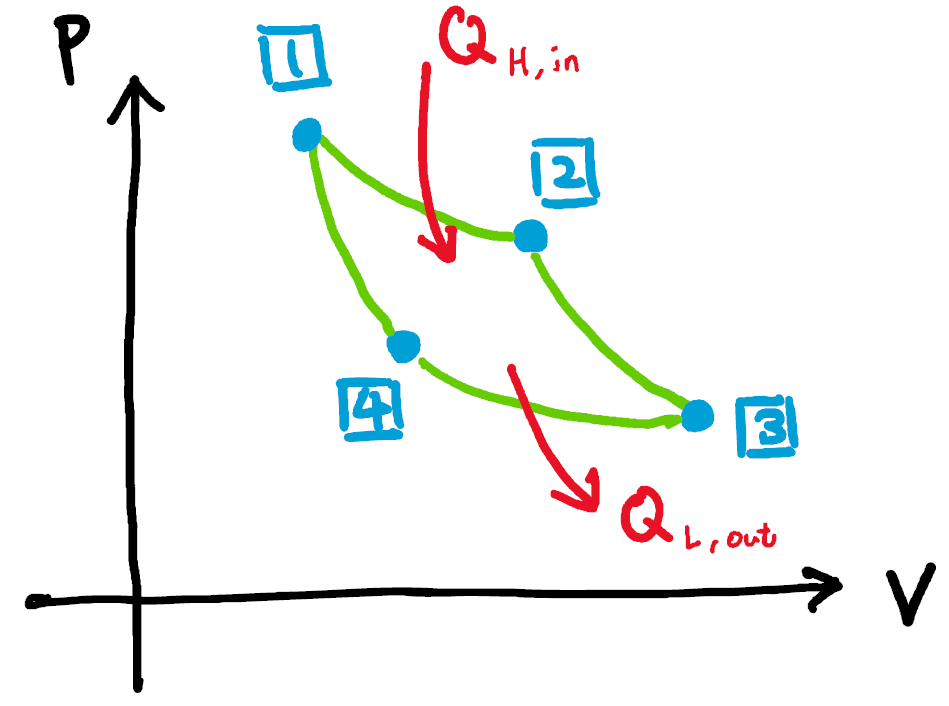
\includegraphics[width=\textwidth]{carnot_cycle_Q}
        \end{minipage}
    \end{center}

    Denote the heat exchange:
    \begin{itemize}
        \item Along \cbox[blue]{1} $\rightarrow$ \cbox[blue]{2} : $Q_{H,\text{in}}$
        = The amount of heat flow into the engine in one cycle.
        
        \item Along \cbox[blue]{3} $\rightarrow$ \cbox[blue]{4} : $Q_{L,\text{out}}$
        = The amount of heat flow out of the engine in one cycle.
    \end{itemize}

    \vskip 1ex
    The efficiency formula of Carnot engine tells that 
    \aleq{
        \eta = 1 - \frac{Q_{L,\text{out}}}{Q_{H,\text{in}}} &= 1 - \frac{T_L}{T_H}\\[1ex]
        %
        \frac{Q_{H,\text{in}}}{T_H} &= \frac{Q_{L,\text{out}}}{T_L}
    }

    Therefore
    \aleq{
        \oint_\text{Carnot} \dd{S} 
        &= \int_\text{Isothermal 1} \frac{\dd{Q}_\green{\text{in}}}{T}
            + \int_\text{Isothermal 2} \frac{\dd{Q}_\green{\text{in}}}{T}\\[1ex]
        %
        &= \frac{Q_{H,\text{in}}}{T_H} + \frac{Q_{L,\text{in}}}{T_L} \\[1ex]
        %
        &= \frac{Q_{H,\text{in}}}{T_H} + \frac{\red{(-1)}Q_{L,\red{\text{out}}}}{T_L}\\[1ex]
        %
        &= 0
    }



    \item Second we show that any arbituary cycle can be approximated and cut into many Carnot cycle.
    
    \begin{center}
        \begin{minipage}{0.28\linewidth}
            \centering
            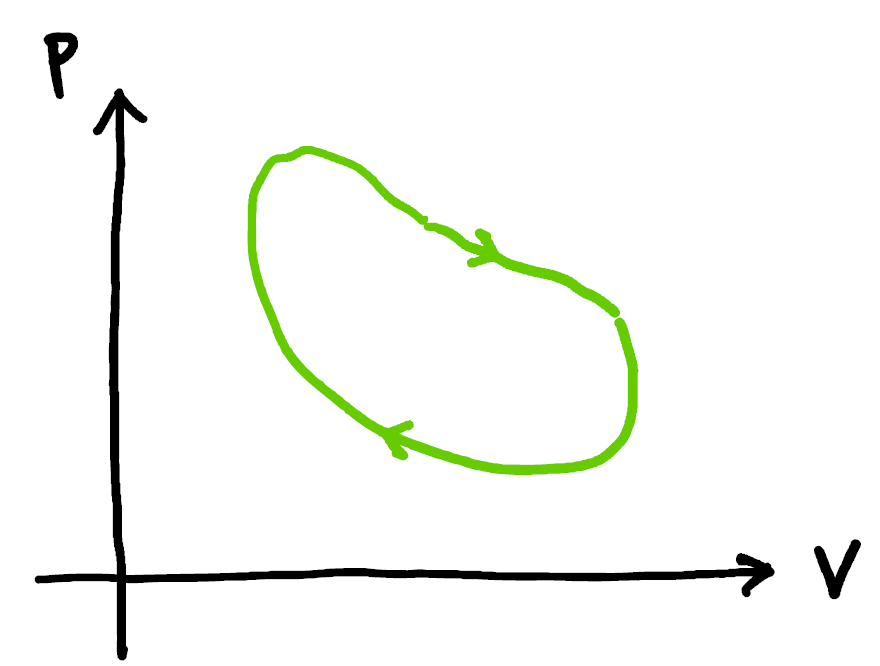
\includegraphics[width=\textwidth]{carnot_overlay1}
        \end{minipage}
        $\xRightarrow{\text{overlay}}$
        \begin{minipage}{0.28\linewidth}
            \centering
            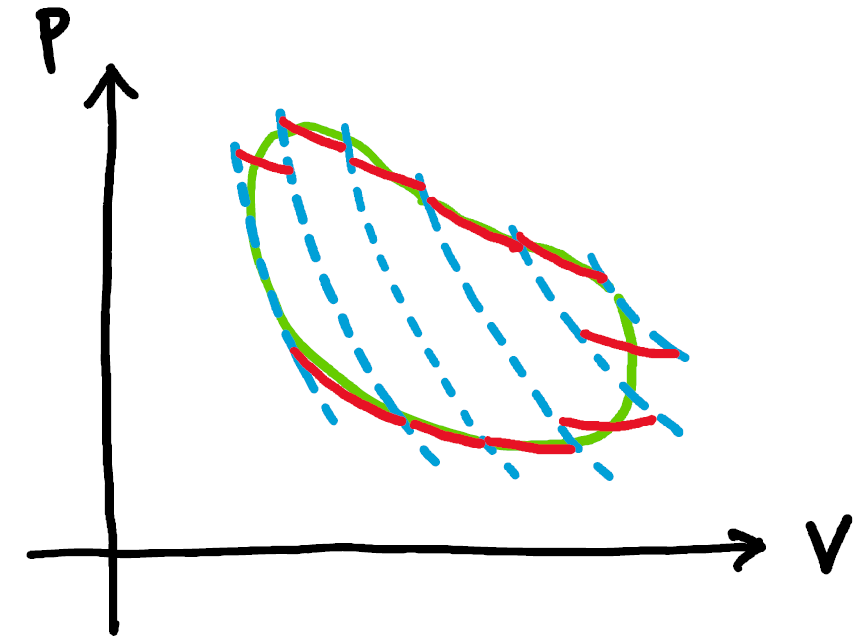
\includegraphics[width=\textwidth]{carnot_overlay2}
        \end{minipage}
        $\xRightarrow{\phantom{\text{over}}}$
        \begin{minipage}{0.28\linewidth}
            \centering
            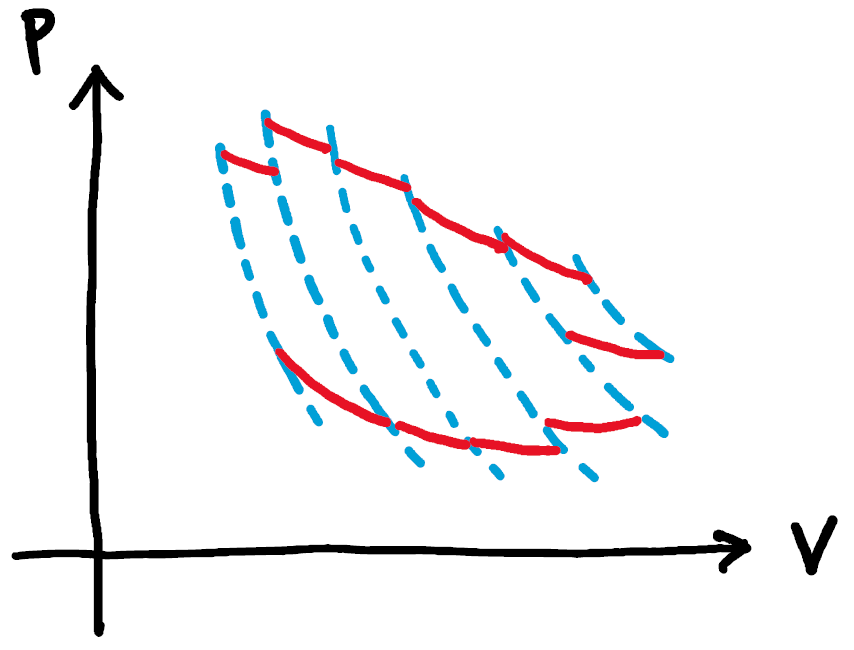
\includegraphics[width=\textwidth]{carnot_overlay3}
        \end{minipage}\\[1em]
        (\blue{Blue = Adiabatic lines}, \red{Red = Isothermal lines})
    \end{center}

    By the property of line integral,
    integrating along the same path but in opposite direction yields negative of the original value,
    just like $\int_a^b f \dd{x} = -\int_b^a f \dd{x}$.

    \begin{center}
        \begin{minipage}{0.4\linewidth}
            \centering
            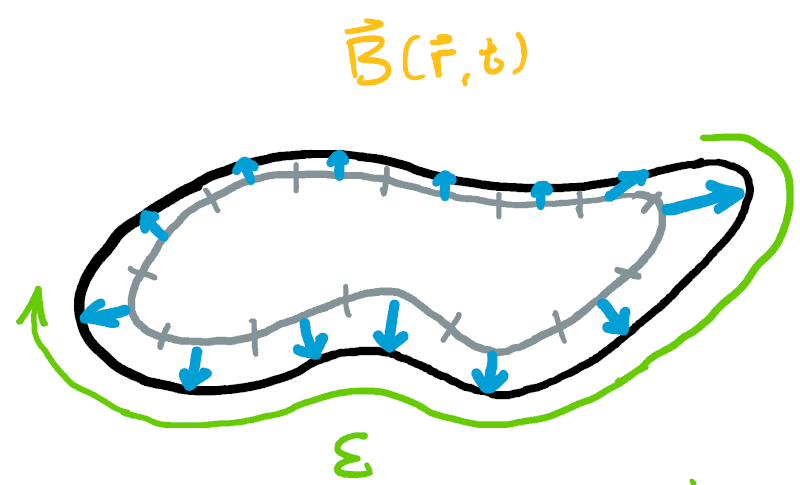
\includegraphics[width=0.75\textwidth]{loop1}\\
            $\displaystyle \oint_\blue{\substack{\text{Blue}\\\text{loop}}} f\dd{\vvec{r}} 
                + \oint_\red{\substack{\text{Red}\\\text{loop}}} f\dd{\vvec{r}}$
        \end{minipage}
        \qquad{\huge $=$}\qquad
        \begin{minipage}{0.38\linewidth}
            \centering
            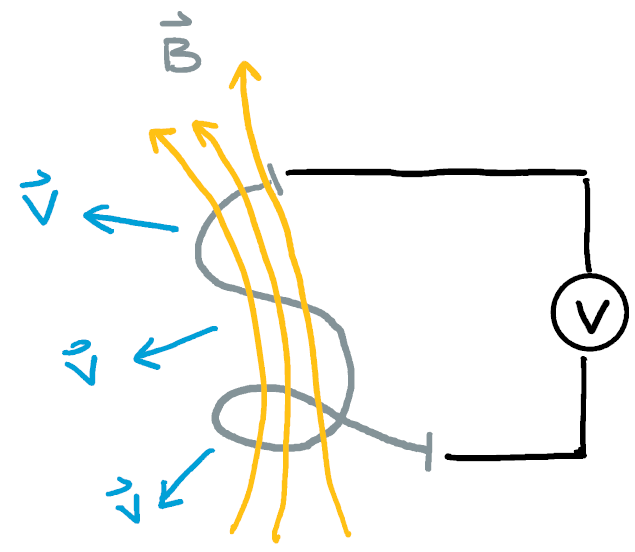
\includegraphics[width=0.75\textwidth]{loop2}\\
            $\displaystyle \oint_{\substack{\text{Black}\\\text{loop}}} f\dd{\vvec{r}}$
        \end{minipage}
    \end{center}

    So we can conclude that $S$ is a state function.
    \aleq{
        \oint_{\substack{\text{Any}\\\text{reversible}\\\text{cycle}}} \dd{S}
        %
        = \sum_{\substack{\text{many many}\\\text{Carnot cycle}}}
        \qty(\oint_\text{Carnot} \dd{S}) 
        %
        = 0
    }

\end{enumerate}

\newpage
\begin{example}
    Consider a simple cycle of ideal gas that only involves 3 states and 3 processes: 
    \begin{center}
    \begin{minipage}{0.4\linewidth}
        \begin{enumerate}
            \item Iso. P (expansion)
            \item Iso. V
            \item Iso. T (contraction)
        \end{enumerate}
    \end{minipage}
    \hspace{0.05\textwidth}
    \begin{minipage}{0.25\linewidth}
        \centering
        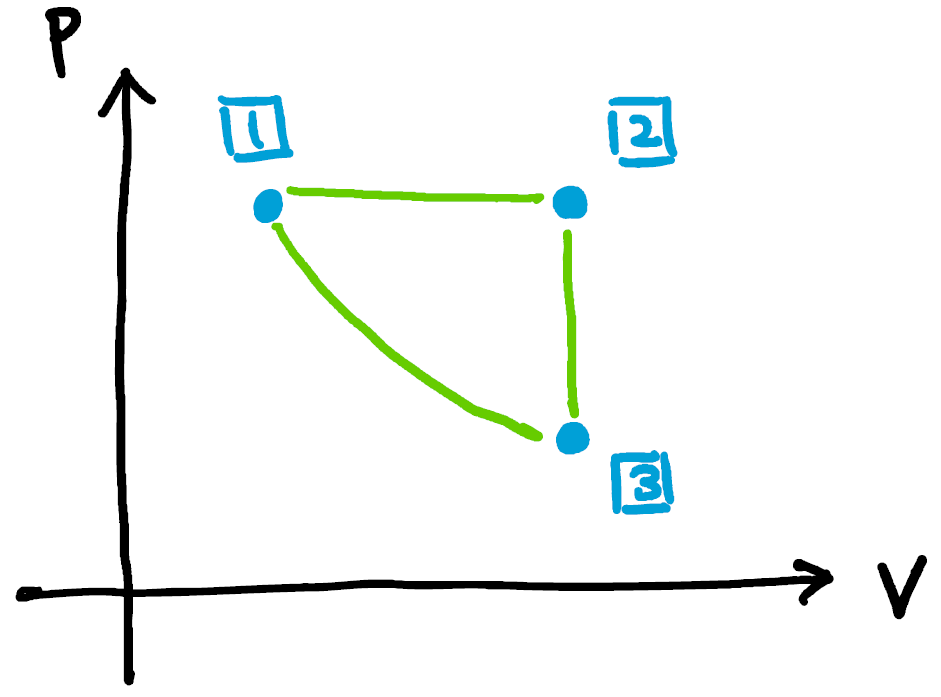
\includegraphics[width=\textwidth]{rand_cycle}
    \end{minipage}
    \end{center}

    We can demonstrate that the entropy change after one cycle is indeed $0$.
    First write down the relations of $P,V,T$ between initial/final states of each process:
    \begin{center}
        \begin{tabular}{>{\centering\arraybackslash}m{3cm} >{\centering\arraybackslash}m{3cm} >{\centering\arraybackslash}m{3cm}}
            & Process & Relation
            \\
            \hline
            \cbox[blue]{1} $\rightarrow$ \cbox[blue]{2}
            & Iso. P
            & $P_1=P_2$
            \\
            \hline
            \cbox[blue]{2} $\rightarrow$ \cbox[blue]{3}
            & Iso. V
            & $V_2 = V_3$
            \\
            \hline
            \cbox[blue]{3} $\rightarrow$ \cbox[blue]{1}
            & Iso. T
            & $T_3=T_1$
        \end{tabular}
    \end{center}
    
    \vskip 1em
    And the entropy change along each process:
    \begin{center}
        \begin{tabular}{>{\centering\arraybackslash}m{2cm} 
            >{\centering\arraybackslash}m{2.5cm} 
            c}
            & Process & $\dd{S}$
            \\
            \hline\\[-3ex]
            \cbox[blue]{1} $\rightarrow$ \cbox[blue]{2}
            & Iso. P
            & $\dfrac{i+2}{2}nR\ln\qty(\dfrac{T_2}{T_1}) \quad \red{> 0}$
            %
            \\[2ex]
            \hline\\[-1ex]
            \cbox[blue]{2} $\rightarrow$ \cbox[blue]{3}
            & Iso. V
            & $\dfrac{i}{2}nR\ln\qty(\dfrac{T_3}{T_2}) \quad \red{< 0}$
            %
            \\[2ex]
            \hline\\[-1ex]
            \cbox[blue]{3} $\rightarrow$ \cbox[blue]{1}
            & Iso. T
            & $nR\ln\qty(\dfrac{V_1}{V_3}) \quad \red{< 0}$
            %
        \end{tabular}
    \end{center}
    
    \vskip 1ex
    Using the state parameters relation and ideal gas property $P_1 = P_2 \Rightarrow \dfrac{T_1}{T_2} = \dfrac{V_1}{V_2}$, 
    \aleq{
        \Delta S &= 
        \dfrac{i+2}{2}nR\ln\qty(\dfrac{T_2}{T_1}) + \dfrac{i}{2}nR\ln\qty(\dfrac{T_3}{T_2}) + nR\ln\qty(\dfrac{V_1}{V_3}) \\[1ex]
        %
        &= \dfrac{i+2}{2}nR\ln\qty(\dfrac{T_2}{T_1}) + \dfrac{i}{2}nR\ln\qty(\dfrac{\red{T_1}}{T_2}) + nR\ln\qty(\dfrac{V_1}{\red{V_2}}) \\[1ex]
        %
        &= \dfrac{i+2}{2}nR\ln\qty(\dfrac{T_2}{T_1}) + \dfrac{i}{2}nR\ln\qty(\dfrac{T_1}{T_2}) + nR\ln\qty(\blue{\dfrac{T_1}{T_2}}) \\[1ex]
        %
        &= 0
    }

    As entropy is a state function, it is guarenteed to be the same after any \cul[red]{cycle of reversible processes}.
\end{example}


\newpage
%%%%%%%%%%%%%%
\subsection{Clausius Theorem}

Entropy is a special state function that when we consider a \cul[red]{closed system} (Energy conserved within) -
no matter how the objects interact (thermal, mechanical, etc.),
the total change in their entropy is always $\geq 0$.
\begin{itemize}
    \item Equality holds if all the interaction processes are reversible.
    \item Becomes inequality if there involve irreversible processes.
\end{itemize}
\aleq{
    \Aboxed{
        \balg{
            \Delta S_\blue{\text{irrev}}
            \ >\ 
            \Delta S_\blue{\text{rev}}
            \ =
            \sum_{\substack{\text{All objects}\\\text{involved in}\\\text{energy exchange}}}
            \int_{\substack{\text{Any}\\\text{\blue{reversible}}\\\text{process}}}
            \frac{\var{Q_\green{\text{in}}}}{T}
            \quad =\ \mstack{\text{\cul[red]{\Large 0}}}
        }
    }
}

This is the \bf{Clausius theorem}. 
The theorem origins from a simple fact - 
thermal interactions (i.e. heat exchange) between two objects occurs only if they have a temperature difference.

\begin{enumerate}
    \item Let the hotter object be at temperature $T_H$ and the colder temperature be at temperature $T_C$.
    We must always have $T_H>T_C$ in order to have heat exchange.

    \item By energy conservation, 
    heat flowing out of the hotter object, $Q_{H,\text{out}}$, must equal to heat flowing into the colder object $Q_{C,\text{in}}$.

\end{enumerate}

Combining the two conditions, 
\vskip -1em
\aleq{
    \frac{Q_{H,\text{out}}}{T_H} 
    &< 
    \frac{Q_{C,\text{in}}}{T_C} \\[1ex]
    %
    \cub[red]{\frac{Q_{H,\text{\red{in}}}}{T_H}}{\substack{\Delta S \text{ of}\\\text{Hotter object}}}
    + 
    \cub[blue]{\frac{Q_{C,\text{in}}}{T_C}}{\substack{\Delta S \text{ of}\\\text{Colder object}}}
    &> 0\\[1ex]
    %
    \Rightarrow\quad \tkn{sum}{\sum_{\substack{\text{All objects}\\\text{involved in}\\\text{energy exchange}}}} 
    \qty(\frac{Q_{\text{in}}}{T}) 
    &>0 
}
\addArrow[red]{sum}{(-6ex,2.5ex)}{}{(0,3ex)}
\addArrow[blue]{sum}{(7ex,2.5ex)}{}{(1ex,3ex)}

As told by Kelvin's statement of \nth{2} law, 
heat flow from hot objects to cold objects are not reversible unless work done is applied.
To reduce the change in entropy, 
we can connect the two objects by a Carnot engine,
splitting the heat transfer process into two steps:

\vskip 1em
\begin{minipage}{0.7\linewidth}
    \begin{enumerate}
    \item \ul{Heat flow from hot object to engine} : 
    Because $Q'_{H,\text{out}} = Q'_{E,\text{in}}$\\ 
    and it requires $T_H > T_{E,H}$ for heat transfer to occur,
    \aleq{
        \frac{Q'_{H,\text{out}}}{T_H} 
        < 
        \frac{Q'_{E,\text{in}}}{T_{E,H}}
    }
    \end{enumerate}
\end{minipage}
\hspace{0.03\textwidth}
\begin{minipage}{0.2\linewidth}
    \centering
    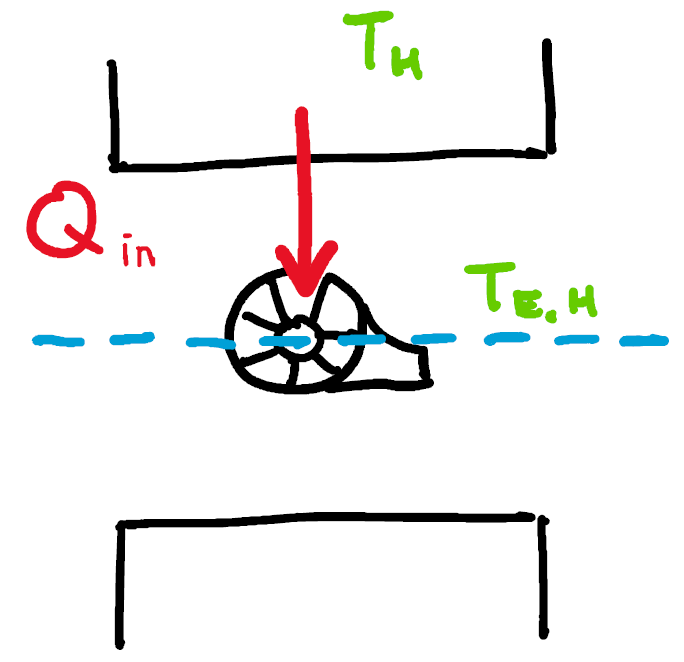
\includegraphics[width=\textwidth]{engine_res1}
\end{minipage}
\\[1em]
\begin{minipage}{0.7\linewidth}
    \begin{enumerate}
    \item[2.] Heat flow from engine to cold object.
    Because $Q'_{E,\text{out}} = Q'_{C,\text{in}}$ and it requires $T_{E,C} > T_C$ for heat transfer to occur,
    \aleq{
        \frac{Q'_{E,\text{out}}}{T_{E,C}}
        < 
        \frac{Q'_{C,\text{in}}}{T_C} 
    }
    \end{enumerate}
\end{minipage}
\hspace{0.03\textwidth}
\begin{minipage}{0.2\linewidth}
    \centering
    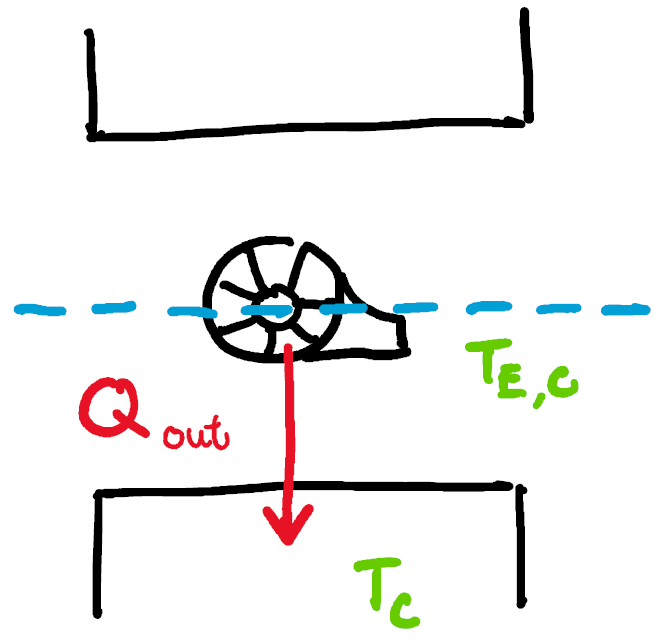
\includegraphics[width=\textwidth]{engine_res2}
\end{minipage}

\vskip 2em
The total entropy change is still $>0$,
but it is smaller than that when engine does not exist:
\aleq{
    0<
    %
    \cub[red]{\frac{Q'_{H,\text{\red{in}}}}{T_H}}{\substack{\Delta S \text{ of}\\\text{Hotter object}}}
    +\quad \cub[green]{\frac{Q'_{E,\text{in}}}{T_{E,H}} + \frac{Q'_{E,\text{\red{in}}}}{T_{E,C}}}{\substack{\Delta S \text{ of}\\\text{Engine}}}
    \quad + \cub[blue]{\frac{Q'_{C,\text{in}}}{T_C}}{\substack{\Delta S \text{ of}\\\text{Colder object}}}
    %
    <\  \frac{Q_{H,\text{\red{in}}}}{T_H}
    + 
    \frac{Q_{C,\text{in}}}{T_C}
}

Because the engine converts part of the heat transfer into W.D.,
this W.D. can be "saved up" and used to revert the heat flow later. 
The system is "less irreversible".

\begin{center}
    \begin{minipage}{0.3\linewidth}
        \centering
        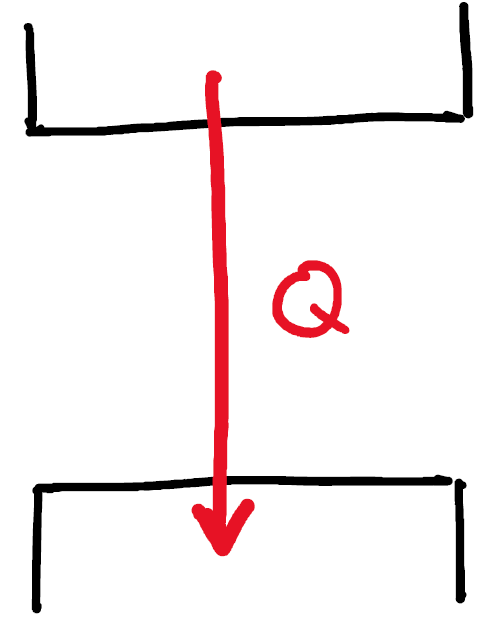
\includegraphics[height=8em]{engine_res3}\\
        Without engine,\\ heat flow irreversibly.
    \end{minipage}
    \hspace{0.05\textwidth}
    \begin{minipage}{0.6\linewidth}
        \centering
        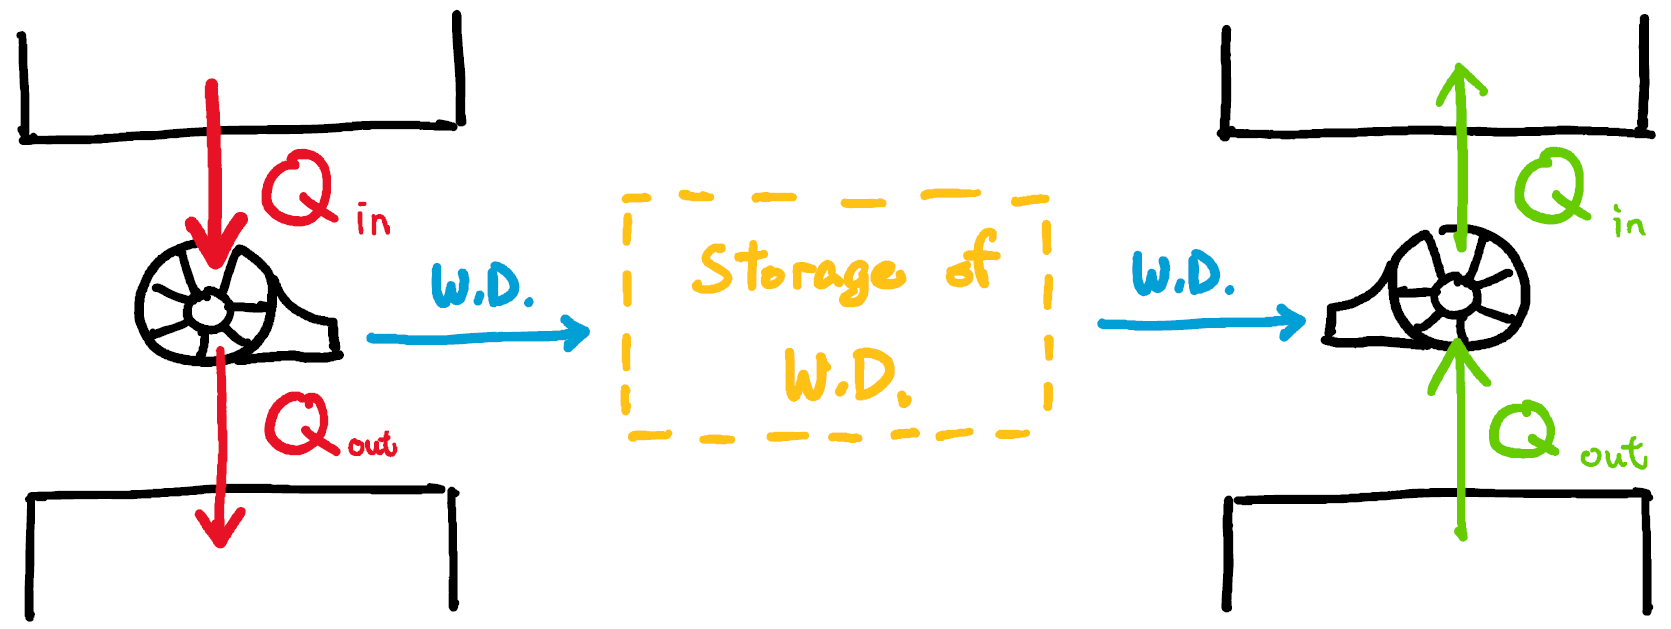
\includegraphics[height=8em]{engine_res4}\\
        With engine, W.D. can be saved up\\
        to reverse heat flow.
    \end{minipage}
\end{center}

Ideally, if
\begin{itemize}
    \item The heat engine is a reversible engine (So $\Delta S = 0$ for the engine), and
    \item $T_H - T_{E,H}$ and $T_{E,C} - T_C$ are infinitestimally small ($\approx 0$),
\end{itemize}

then the total $\Delta S=0$ and the work done extracted by the engine can be used to invert the heat flow completely.
Only then we can say the system is reversible.



\vskip 2em
\begin{example}
    Water can enter a supercool phase under certain condition.
    In this phase, the water is below $0^\circ$C under atmospheric pressure, 
    but remains in liquid state. 
    This state is "meta-stable" - if the water received a shock, 
    the water will freeze into ice spontaneously.\\
    
    You can watch a video demonstration \href{https://www.youtube.com/watch?v=kEHdyiBMgAg}{here}.\\
    
    We can show that this freezing process is an irreversible process
    by computing the entropy change.\\

    Given the following data:
    \begin{itemize}
        \item Both the supercooled water and ice are at $-10^\circ$C $= 263.15$ K.
        \item Heat capacity under constant pressure of ice $ C_{P,\text{I}}= 2100$ J/K/kg.
        \item Heat capacity under constant pressure of water $ C_{P,\text{W}}= 4184$ J/K/kg.
        \item Latent heat of fusion of water $L = 334000$ J/kg.
    \end{itemize}

    \vskip 1ex
    We can form a cycle with two processes:
    \begin{itemize}
        \item \ul{Ice to Supercooled water} : With the help of a refridgerator. Reversible.
        \item \ul{Supercooled water to ice} : Spontaneously freezing.
    \end{itemize}

    \begin{center}
        \begin{minipage}{0.7\linewidth}
            \centering
            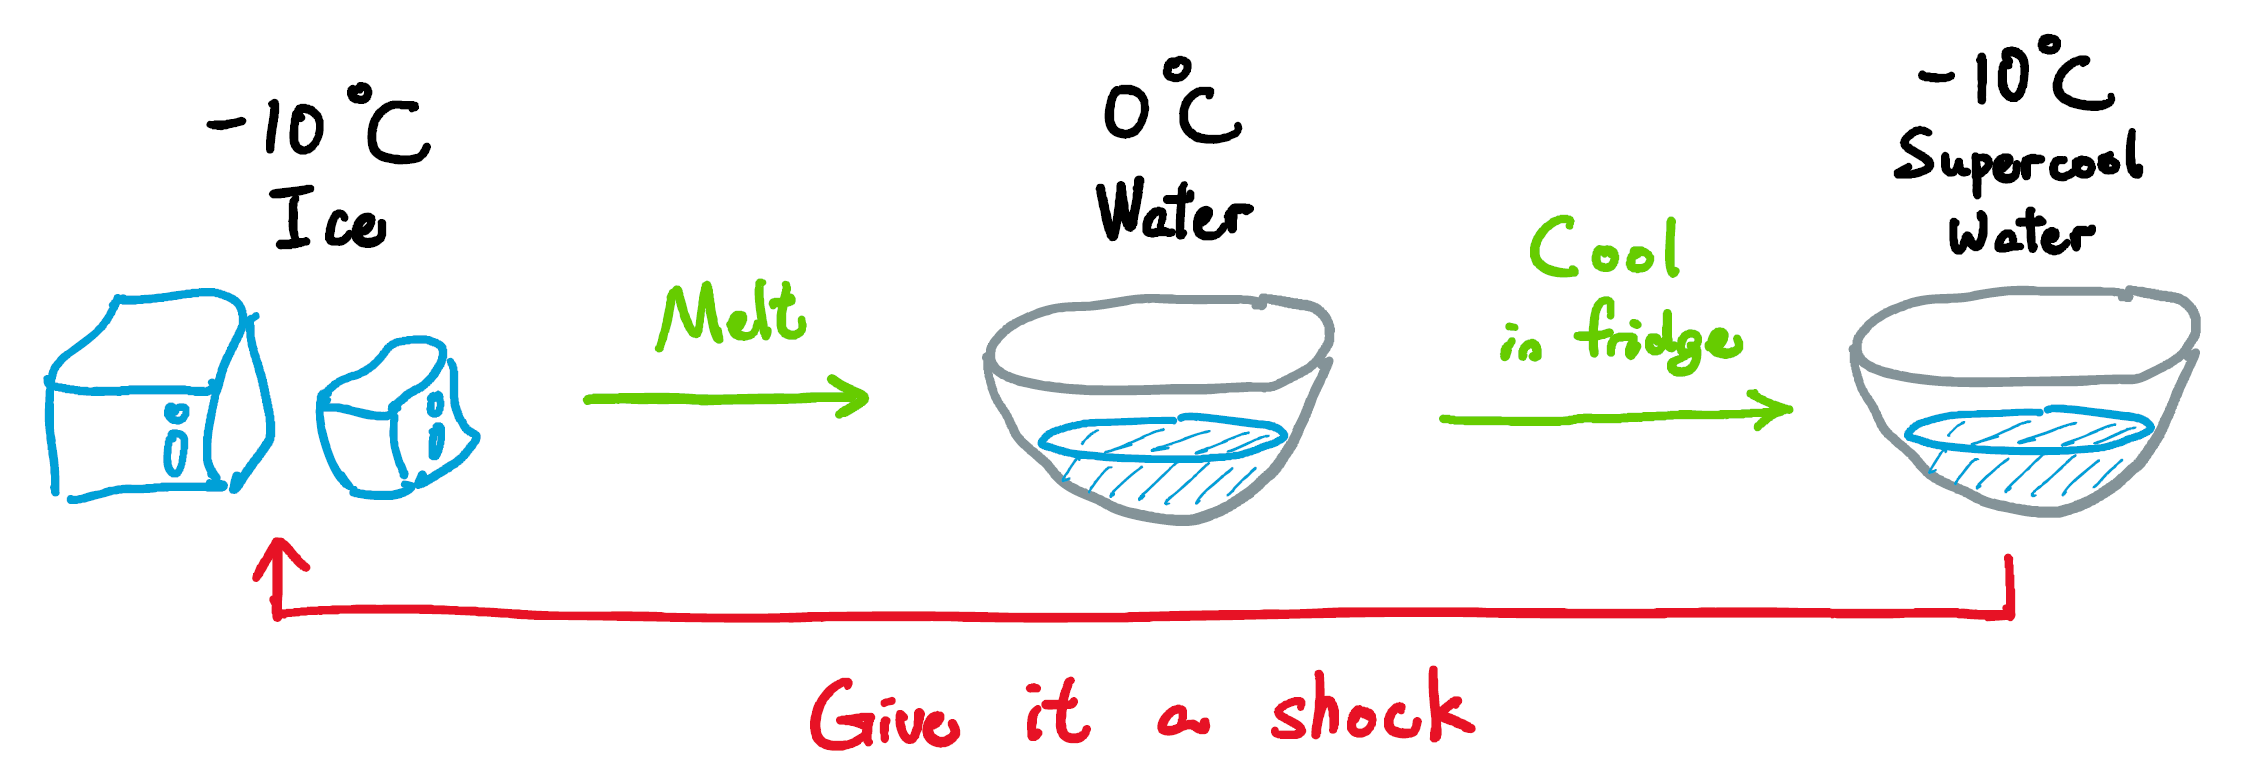
\includegraphics[width=\textwidth]{supercool}
        \end{minipage}
    \end{center}

    Note that in the melting/freezing process, 
    heat exchange occurs between the ice/supercooled water and \cul[red]{the envirnoment}.
    When calculating total entropy change,
    we must also consider the change in the environment.


    \begin{enumerate}
        \item The reversible path from ice to supercooled water involving using a refridgerator, 
        which absorb energy from the environment to do work on the ice.
        The change in entropy of the ice is
        \aleq{
            \Delta S_\text{ice, \red{rev}} 
            &= \Delta S_\text{heat up} + \Delta S_\text{melting} + \Delta S_\text{cool to water}\\
            %
            &= \int_{263.15}^{273.15} \frac{C_{P,I}}{T}\dd{T} + \frac{L}{273.15} + \int_{273.15}^{263.15} \frac{C_{P,W}}{T}\dd{T}\\
            %
            &\approx 1145
        }
        
        This is a reversible process.
        The total entropy change of (ice + environment) must be $0$.
        \aleq{
            \Delta S_\text{envr, \red{rev}} = - \Delta S_\text{ice, \red{rev}}  = -1145
        }
        
        \item After spontaneous freezing, 
        the ice/supercooled water has returned to its original state.
        Because entropy is a state function, 
        we know that the entropy must also return to its original value. 
        So the change in this process is
        \aleq{
            \Delta S_\text{ice, \red{irrev}} = - \Delta S_\text{ice, \red{rev}} = -1145 
        }

        However, the process of energy exchange with the environment is not the same as when operating a refridgerator. 
        \red{All because there is no W.D. involve}. 
        Temperature of the environment remains at $263.15$ K throughout the process. 
        \aleq{
            \Delta S_\text{envr, \red{irrev}} 
            &= \frac{C_{P,I}\times 10 + L - C_{P,W}\times 10}{263.15}\\
            %
            &\approx 1190
        }
    \end{enumerate}

    So there is an increase of entropy $1190-1145 \approx 45$ J/K/kg 
    when supercooled water of $-10^\circ$C spontaneously freezes.

\end{example}

%%%
\theend
\end{document}